%% Computer Methods and Programs in Biomedicine -- Elsevier elsarticle package
%% Created from paper/sections/ for Overleaf upload.
%% First submission: preprint layout is acceptable per Elsevier guidance.
\documentclass[preprint,12pt,3p,times]{elsarticle}

\usepackage[T1]{fontenc}
\usepackage[utf8]{inputenc}
\usepackage{amsmath,amssymb}
\usepackage{graphicx}
\usepackage{booktabs}
\usepackage{adjustbox}
\usepackage{xcolor}
\usepackage{textcomp}
\usepackage{float}
\newfloat{algorithm}{htbp}{loa}
\floatname{algorithm}{Algorithm}
\usepackage[expansion=false,protrusion=true]{microtype}
\usepackage{xurl}
\usepackage{hyperref}
\hypersetup{hidelinks,breaklinks=true,pdfauthor={},pdfcreator={}}
\urlstyle{tt}
% Allow slightly stretchy paragraphs instead of margin overflow.
\emergencystretch=3em
\tolerance=2000
\hbadness=10000
\hyphenpenalty=400
\exhyphenpenalty=100
% Soft hyphenation hints for dense technical prose
\hyphenation{phar-ma-co-dy-nam-i-cal-ly Chem-BER-Ta Done-pezil Mem-an-tine
CAU-EEG Alz-hei-mer con-nec-tiv-i-ty}

\journal{Computer Methods and Programs in Biomedicine}

\bibliographystyle{elsarticle-num}

\begin{document}

\begin{frontmatter}

\title{SEME: A Decoupled Evaluation Protocol for
Literature-Constrained EEG--Drug Generators}

\author{Authors to be completed at submission}

\begin{abstract}
\noindent\textbf{Background and Objective:} Chemistry-conditioned EEG generators are often scored with conflated endpoints. We introduce SEME (Signed concordance, Effect-vector fidelity, Magnitude transfer, Encoding retention), a formal evaluation protocol that scores those axes separately for literature-constrained EEG--drug generators, demonstrated on a pharmacodynamically penalized CVAE for Donepezil and Memantine.

\noindent\textbf{Methods:} Under SEME, a constrained CVAE ($N{=}66$; 2185-D EEG features; frozen ChemBERTa embeddings) used subject-level five-fold splits. External cohorts lacked paired pre/post-drug EEG, so signed concordance and continuous effect-vector $r$ were scored against the training constrained signature on TUH, OSF, and P-ADIC. Core controls were matched unconstrained twins, a prior-only signed effect (circularity budget), linear imitation on CVAE-simulated targets, fold/seed sensitivity, and CAUEEG encoding probes against theta/alpha and packed 2185-D logistic references, with paired DeLong tests on stored out-of-fold scores.

\noindent\textbf{Results:} On the locked sign endpoint, constrained twins reached 10/10 agreement on TUH, OSF, and P-ADIC while matched unconstrained twins failed (3/10, 4/10, 4/10). Prior-only already reached 10/10 signs at mean $r{=}0.636$, so binary signs are partly prior-recoverable. Continuous $r$ at the locked fold-0 seed-42 checkpoint was high ($0.908$/$0.851$/$0.918$) but checkpoint-specific (five-fold means $0.385$/$0.371$/$0.372$; non-42 seeds typically 0.08 to 0.43). Magnitude did not diagnose reliably. Encoding bake-off placed latent ROC-AUC $0.579$ below theta/alpha $0.675$ and a 2185-D logistic reference of $0.699$ (best nested-head OOF AUC $0.593$; DeLong $p{<}0.001$ vs 2185-D).

\noindent\textbf{Conclusions:} SEME shows that constrained sign concordance is the more reproducible external finding in this battery, that continuous fidelity is checkpoint-specific, that prior-only bounds circularity for signs, and that residual latent diagnostic signal sits below classical feature references. The study supports a scoped measurement framework, not post-dose pharmacodynamic validation, seed-stable continuous fidelity, or standalone external diagnosis.
\end{abstract}

\begin{keyword}
SEME evaluation protocol \sep pharmacodynamically constrained CVAE \sep EEG-drug simulation \sep external signature assessment \sep encoding-level attenuation \sep reproducibility
\end{keyword}

\begin{highlights}
\item SEME protocol separates signs, continuous r, magnitude, and encoding.
\item Constrained signs beat unconstrained; locked high r is checkpoint-specific.
\item Prior-only reaches 10/10 signs (mean r=0.636); circularity budget made explicit.
\item No paired post-dose EEG; endpoint is signature concordance, not PD validation.
\item Latent AUC 0.579 vs theta/alpha 0.675 and 2185-D 0.699; head OOF 0.593.
\end{highlights}

\begin{graphicalabstract}
\centering
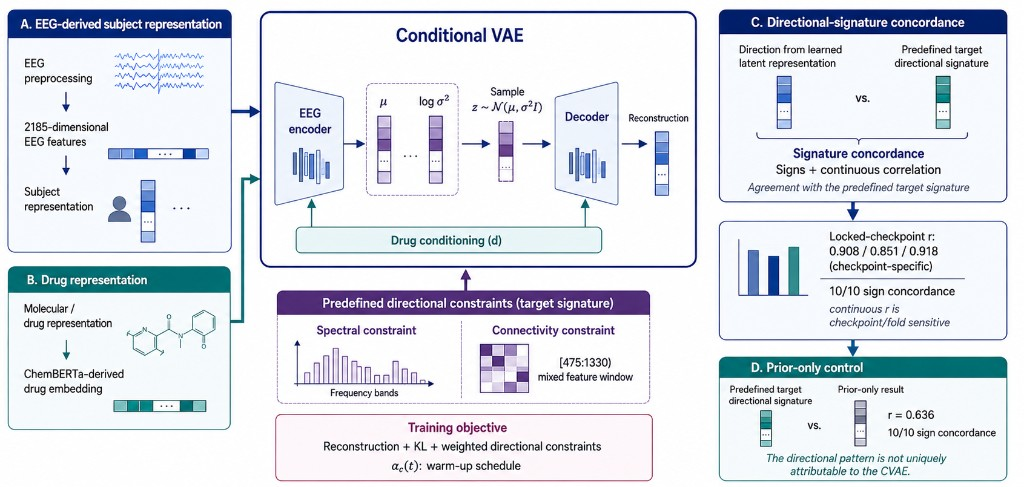
\includegraphics[width=\textwidth]{figures/graphical_abstract.png}
\\[0.4em]
{\footnotesize Direction scoring uses the 2185-D feature-space drug-minus-baseline effect vector, not CVAE latent means. SEME treats signs, continuous $r$, magnitude, and encoding as separate axes.}
\end{graphicalabstract}

\end{frontmatter}

\section{Introduction}
\label{sec:introduction}
Chemistry-conditioned generative models are increasingly used to simulate how a named intervention would change physiological features. Signed concordance, continuous effect-vector fidelity, magnitude transfer, and residual encoding must be scored separately; conflating them invites failure modes in which one metric succeeds while another fails. Conditional variational autoencoders (CVAEs) make that risk concrete, because reconstruction, perturbation fidelity, and downstream classification need not move together \citep{Kingma2014VAE,Higgins2017betaVAE,Rampasek2019DrVAE,Lotfollahi2019scGen}. A formal evaluation design that measures those quantities on the same EEG-drug generator remains scarce.

Closest methods address parts of the problem: standard and \(\beta\)-VAEs \citep{Kingma2014VAE,Higgins2017betaVAE}, molecular or single-cell perturbation models \citep{Rampasek2019DrVAE,Lotfollahi2019scGen}, and diagnosis-oriented EEG twins such as DADD \citep{Amato2025DADD,Amato2026DADDnpj}. Alzheimer's disease (AD) drug response is a natural stress test given heterogeneous AChEI benefit and established EEG markers of cholinergic change \citep{Lu2020DonepezilGenetics,Pozzi2022AChEIPredictors,Jeong2004EEGreview,Cassani2018EEGADReview,Babiloni2006DonepezilEEG}. Those facts motivate constrained in silico simulation of Donepezil and Memantine. They do not license treating every latent as a clinical biomarker or every signature match as post-dose validation.

This paper contributes \textbf{SEME} (Signed concordance, Effect-vector fidelity, Magnitude transfer, Encoding retention): a formal evaluation protocol for literature-constrained, chemistry-conditioned EEG generators. The worked example is a pharmacodynamically penalized CVAE with 2185-D resting EEG features and frozen ChemBERTa embeddings for Donepezil and Memantine \citep{Chithrananda2020ChemBERTa,Winblad2007Memantine}. Under SEME we score signed concordance and continuous effect-vector correlation on Temple University Hospital (TUH) EEG \citep{Obeid2016TUH}, an Open Science Framework (OSF) AD/healthy control set, and P-ADIC AD/healthy control recordings \citep{Shor2021PADIC}; magnitude diagnosis across an escalating sequence that adds CAUEEG Normal/MCI/Dementia strata \citep{Kim2023CAUEEG}; and CAUEEG encoding probes against spectral and raw-feature references. Training features use OpenNeuro ds004504 \citep{Miltiadous2023OpenNeuro}. Domain shift is part of the test \citep{Gulrajani2021DomainShift}.

The paper does not claim clinical validation, pharmacological efficacy, post-dose digital-twin validation, diagnostic superiority, ChemBERTa chemical generalization, or constraint-caused diagnostic compression. The contributions are:

\begin{itemize}
  \item SEME as a decoupled protocol with matched unconstrained, prior-only (circularity budget), linear imitation, five-fold, and multi-seed controls as core method.
  \item Constrained twins exceed unconstrained twins on the locked sign endpoint (10/10 versus 3/10--4/10 on TUH/OSF/P-ADIC), while continuous \(r\) at locked fold-0 seed-42 (\(0.908/0.851/0.918\)) is fold- and seed-sensitive (five-fold means \(0.385/0.371/0.372\); non-42 seeds typically 0.08 to 0.43) and prior-only already reaches 10/10 signs at mean \(r = 0.636\).
  \item Magnitude does not diagnose reliably across four escalating external tests, and an encoding bake-off retains only partial label information in \(\mu_{\mathrm{base}}\) (latent ROC-AUC 0.579; best head OOF 0.593) below theta/alpha 0.675 and a 2185-D logistic feature-space reference of 0.699.
\end{itemize}

Section 2 defines the case-study twin and SEME endpoints. Section 3 applies the protocol. Section 4 interprets incremental value and dissociation. Section 5 concludes.


\section{Methods}
\label{sec:methods}
This section defines the case-study generator, constraints, cohorts, and the SEME endpoint families (Signed concordance, Effect-vector fidelity, Magnitude transfer, Encoding retention). Paired post-dose EEG is not part of the design. Configuration keys, scripts, and artifact paths are listed in Supplementary Material S1.

\subsection{Architecture and pharmacodynamic penalties}

The twin is a pharmacodynamically constrained CVAE (\texttt{constrained\_mlp}): MLP encoders, no graph EEG encoder, no cross-attention, constrained loss enabled. Input EEG is a packed 2185-D vector for 19 standard 10-20 channels (PSD \([0,380)\), band powers \([380,475)\), interleaved coherence/PLV connectivity \([475,2185)\)). \(L_{\mathrm{band}}\) uses delta through beta slices; \(L_{\mathrm{conn}}\) uses window \([475,1330)\), which mixes early-band coherence and PLV under the interleaved flatten (S1). Layer widths and parameter count are in Table~\ref{tab:architecture}. Fig.~\ref{fig:architecture} summarizes data flow.

\begin{figure*}[!t]
\centering
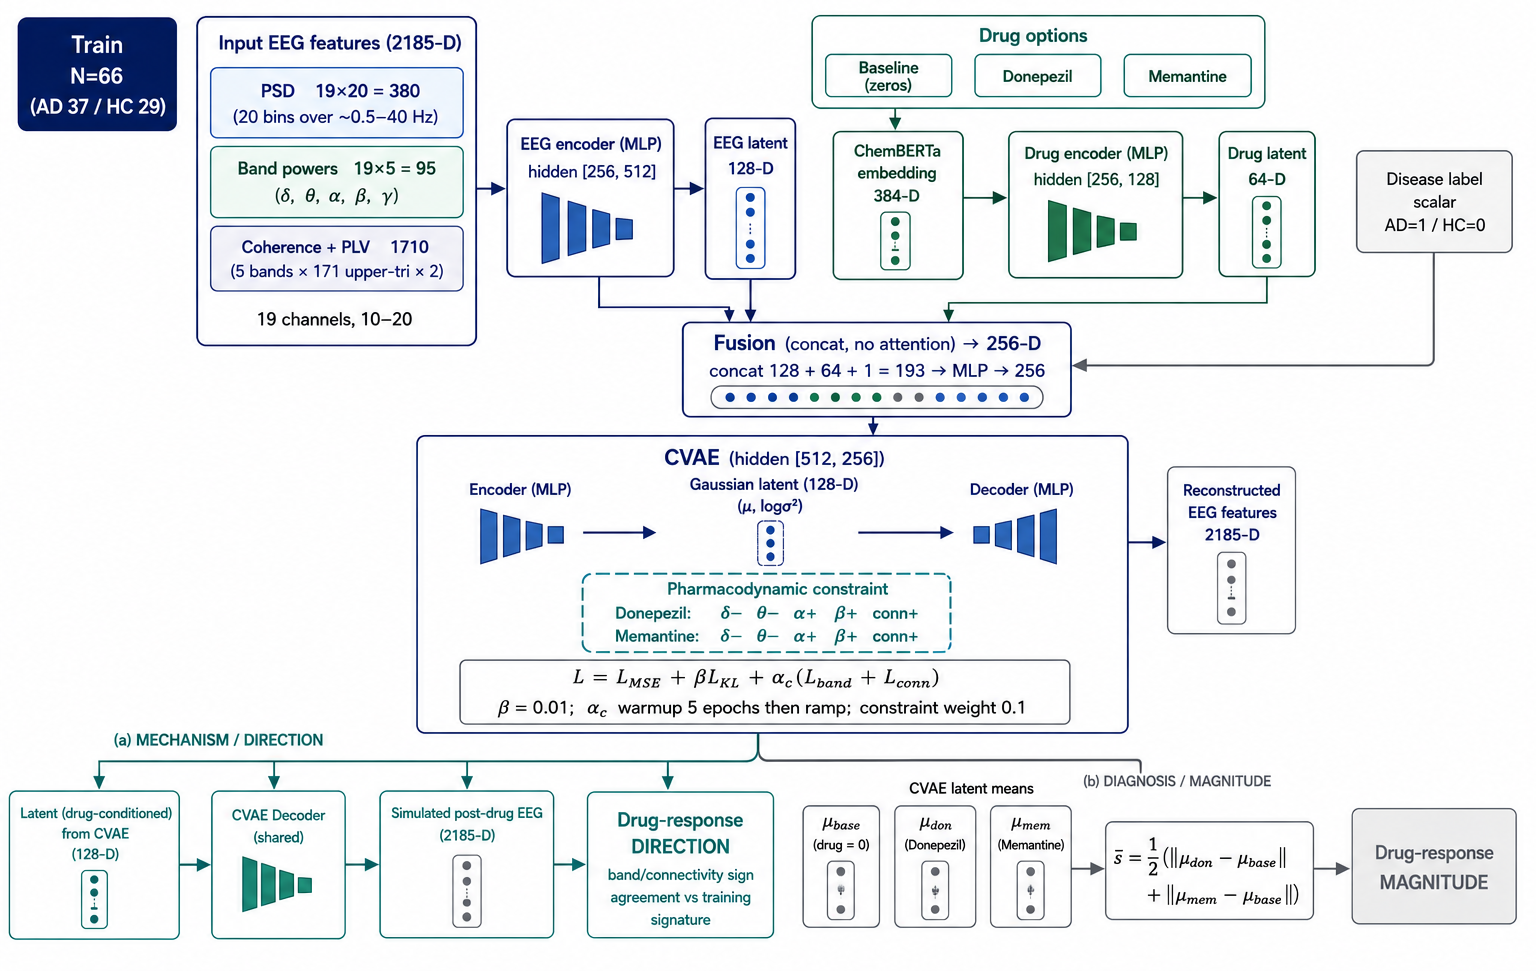
\includegraphics[width=\textwidth]{figures/fig1_architecture.png}
\caption{Architecture of the pharmacodynamically constrained conditional variational autoencoder (CVAE). Resting-state EEG features (2185-D) and ChemBERTa drug embeddings are encoded and fused with a disease label, then mapped by a CVAE whose training includes pharmacodynamic band and connectivity constraints. Training cohort: $N = 66$ (AD 37 / HC 29).}
\label{fig:architecture}
\end{figure*}


The EEG encoder maps structured tensors to a 128-D EEG latent. The drug encoder maps a frozen 384-D ChemBERTa embedding (\texttt{DeepChem/ChemBERTa-77M-MLM}) to a 64-D drug latent; ChemBERTa is not trained. Fusion concatenates EEG latent, drug latent, and a scalar disease label (AD = 1, HC = 0) into a 256-D representation. The CVAE encoder outputs a diagonal Gaussian in 128 dimensions with reparameterization
\begin{equation}
z = \mu + \exp(\tfrac{1}{2}\log\sigma^2)\odot\varepsilon, \qquad \varepsilon\sim\mathcal{N}(0,I).
\label{eq:reparam}
\end{equation}
The decoder reconstructs the 2185-D vector. At inference, baseline uses a zero drug vector; Donepezil/Memantine use their ChemBERTa embeddings. \(\mu_{\mathrm{base}}\) denotes the zero-drug latent mean.

Signed literature priors enter as penalty terms added to reconstruction and KL \citep{Babiloni2006DonepezilEEG,Jeong2004EEGreview,Winblad2007Memantine,Rive2013Memantine}:

\begin{itemize}
  \item Donepezil: \(\delta-0.15\), \(\theta-0.20\), \(\alpha+0.25\), \(\beta+0.10\), connectivity \(+0.20\)
  \item Memantine: \(\delta-0.10\), \(\theta-0.15\), \(\alpha+0.10\), \(\beta+0.05\), connectivity \(+0.15\)
\end{itemize}

With reconstruction \(L_{\mathrm{MSE}}=\mathrm{mean}((\hat{x}-x)^2)\), KL weight \(\beta=0.01\), band ReLU penalties \(L_{\mathrm{band}}\), connectivity non-decrease penalty \(L_{\mathrm{conn}}\) (prior connectivity magnitudes are stored but not multiplied into \(L_{\mathrm{conn}}\)), and schedule \(\alpha_c(t)\) rising from 0 after a 5-epoch warmup to \(\alpha_c^{\star}=0.1\), the total loss is
\begin{equation}
L = L_{\mathrm{MSE}} + \beta L_{\mathrm{KL}} + \alpha_c(t)\,L_{\mathrm{band}} + \alpha_c(t)\,L_{\mathrm{conn}}.
\label{eq:total}
\end{equation}
The KL term against \(\mathcal{N}(0,I)\) is
\begin{equation}
L_{\mathrm{KL}} = \frac{1}{B}\sum_{i=1}^{B}\Bigl(-\tfrac{1}{2}\sum_{k=1}^{128}\bigl(1+\log\sigma^2_{ik}-\mu_{ik}^2-\exp(\log\sigma^2_{ik})\bigr)\Bigr).
\label{eq:kl}
\end{equation}
For band \(b\in\{\delta,\theta,\alpha,\beta\}\) with reconstructed change \(\Delta_b\) versus baseline and prior \(\pi_b\),
\begin{equation}
L_{\mathrm{band}} = \sum_{b}|\pi_b|\,\mathrm{ReLU}\bigl(-\mathrm{sign}(\pi_b)\,\Delta_b\bigr),
\label{eq:band}
\end{equation}
and with connectivity-window change \(\Delta_c\),
\begin{equation}
L_{\mathrm{conn}} = \mathrm{ReLU}(-\Delta_c).
\label{eq:conn}
\end{equation}
The implemented schedule is
\begin{equation}
\alpha_c(t)=\begin{cases}
0 & t < T_w,\\
\alpha_c^{\star}\min\bigl(1,(t-T_w)/5\bigr) & t \ge T_w,
\end{cases}
\label{eq:alpha}
\end{equation}
with \(T_w=5\). Algorithm~\ref{alg:train} summarizes training.
\begin{algorithm}[H]
\caption{Training procedure for the pharmacodynamically constrained CVAE.}
\label{alg:train}
\small
\textbf{Input:} packed EEG features $x\in\mathbb{R}^{2185}$ (PSD, band powers, interleaved coherence/PLV); ChemBERTa embedding $d\in\mathbb{R}^{384}$; disease label $y\in\{0,1\}$; subject-level baseline features $x^{\mathrm{base}}$; priors $\pi$ from \texttt{get\_eeg\_effect\_prior}; $\beta=0.01$; $\alpha_c^{\star}=0.1$; $T_w=5$; Adam hyperparameters.\\
\textbf{Output:} checkpoint minimizing validation total loss.\\[0.4em]
\textbf{Training} (subject-level 5-fold; within-fold 10\% validation). For each epoch $t=0,\ldots,T-1$ and each minibatch:
\begin{enumerate}
  \setlength{\itemsep}{0.15em}
  \item Flatten EEG tensors to $x$ with the same packing as the decoder target.
  \item Encode EEG: $h_{\mathrm{eeg}}=\mathrm{EEGEncoder}(\mathrm{PSD},\mathrm{band},\mathrm{coh},\mathrm{PLV})$.
  \item Encode drug: $h_{\mathrm{drug}}=\mathrm{DrugEncoder}(d)$ (384-D ChemBERTa; enhanced 416-D prior concatenation is off for this variant).
  \item Fuse: $h=\mathrm{Fusion}(h_{\mathrm{eeg}},h_{\mathrm{drug}},y)$.
  \item CVAE encode: $(\mu,\log\sigma^2)=\mathrm{Enc}(h)$.
  \item Reparameterize: $z=\mu+\exp(\tfrac12\log\sigma^2)\odot\varepsilon$, $\varepsilon\sim\mathcal{N}(0,I)$.
  \item Decode: $\hat{x}=\mathrm{Dec}([z; h_{\mathrm{drug}}; y])$ (linear output, no output activation).
  \item $L_{\mathrm{MSE}}=\mathrm{mean}((\hat{x}-x)^2)$; $L_{\mathrm{KL}}$ as in Eq.~(\ref{eq:kl}).
  \item If the batch item is not baseline, compute $L_{\mathrm{band}}$ and $L_{\mathrm{conn}}$ vs $x^{\mathrm{base}}$ (Eqs.~(\ref{eq:band})--(\ref{eq:conn})); else both are 0.
  \item Set $\alpha_c(t)$ from Eq.~(\ref{eq:alpha}); form $L$ (Eq.~(\ref{eq:total})). Unique \texttt{drug\_id} subsets are scored separately and summed with batch-fraction weights.
  \item Backpropagate $L$ and take one Adam step.
\end{enumerate}
After each epoch, record train/val losses. Save the fold checkpoint with the lowest validation total loss.\\[0.3em]
\textbf{External evaluation} (not used for the Adam step): freeze the locked fold-0 checkpoint; simulate Donepezil/Memantine feature effects; score direction, magnitude, and encoding probes on held-out cohorts.
\end{algorithm}

Exact index slices and packing notes are in S1.

\subsection{Training cohort, freeze, and sensitivity protocol}

Training features come from resting-state EEG for 66 subjects (AD 37, HC 29; OpenNeuro ds004504). Preprocessing uses FIR 0.5-40 Hz, notch 50 Hz on the training path, FastICA with empty default exclusion, 4 s epochs at 90% overlap, and per-subject z-scoring before Welch/connectivity (S1). Features are 500 Hz spectral/connectivity packs. \(N=66\) is small relative to 2185-D inputs and multilayer capacity; primary claims are therefore external assessments, not training-set diagnosis.

Splits are subject-level stratified 5-fold (\texttt{random\_state=42}); within-fold validation is 10%. External cohorts are never in the training loop. Optimization uses Adam (\(10^{-4}\), weight decay \(10^{-5}\)), batch size 16, 100 epochs. Checkpoint selection minimizes internal validation total loss. The locked alias is fold-0 seed-42 epoch 99 (val total 0.0241). External \(r\), signs, and AUCs are post-freeze assessments, not selection criteria. The freeze is a documented project rule, not independently auditable preregistration. Training-seed sensitivity holds fold membership fixed (\texttt{split\_seed=42}) and varies \texttt{train\_seed} over \(\{42,7,21,123,2024\}\). Compute summary is in Table~\ref{tab:compute}.

\subsection{External cohorts}

Cohorts were introduced so each answered a doubt left by the previous setting (Table~\ref{tab:datasets}).
% Table 1 -- External assessment datasets (fit page width)
% Caption placement: ABOVE the tabular (Elsevier convention).
% Requires: booktabs, adjustbox
\begin{table*}[!t]
\centering
\footnotesize
\setlength{\tabcolsep}{3pt}
\caption{External EEG datasets used for escalating external assessment of the constrained twin.
Sampling rates list native acquisition then the common 500\,Hz analysis rate.
Roles follow the Results narrative sequence.}
\label{tab:datasets}
\begin{adjustbox}{max width=\textwidth}
\begin{tabular}{@{}llp{2.2cm}p{2.4cm}p{2.5cm}p{1.9cm}p{2.4cm}@{}}
\toprule
Dataset & N & Groups & Labels & Sampling rate & Montage & Role \\
\midrule
TUH & 200 & Abn 131 / Nor 69 & Abnormal vs normal & Mixed EDF $\rightarrow$ 500\,Hz & 19ch 10--20 & First external; proxy labels \\
OSF & 92 & AD 80 / HC 12 & Folder AD vs HC & 256 $\rightarrow$ 500\,Hz & 19ch 10--20 & AD/HC; small HC \\
P-ADIC & 145 & AD 49 / HC 96 & NIA-AA AD vs HC & 200/500 $\rightarrow$ 500\,Hz & 19ch 10--20 & Larger AD/HC; null check \\
CAUEEG & 1122 & Nor 436 / MCI 395 / Dem 291 & Normal / MCI / Dementia & 200 $\rightarrow$ 500\,Hz & 19ch AVG 10--20 & Large-N; encoding \\
\bottomrule
\end{tabular}
\end{adjustbox}
\end{table*}


\begin{itemize}
  \item \textbf{TUH} (\(n=200\); abnormal 131 / normal 69): locked features use \texttt{crop\_seconds=60.0} and \texttt{apply\_ica=false} in \texttt{processing\_report.json}; current script default \texttt{CROP\_SECONDS=320.0} was not used to regenerate locked results.
  \item \textbf{OSF} AD/HC (\(n=92\); HC \(n=12\)).
  \item \textbf{P-ADIC} AD/HC (\(n=145\)) \citep{Shor2021PADIC}.
  \item \textbf{CAUEEG} Normal/MCI/Dementia (1122 features OK) for magnitude and encoding \citep{Kim2023CAUEEG}.
\end{itemize}
Direction tests use TUH, OSF, and P-ADIC. CAUEEG was not required for the locked 10/10 direction claim.

\subsection{Evaluation endpoints and statistics}

No paired pre/post-dose EEG is available. Direction measures concordance with the \textbf{training constrained signature}, a prior-shaped model-derived reference. That circularity is intentional and bounded by controls: prior-only (constant literature-signed effect; mean \(r=0.636\), 10/10), matched unconstrained CVAE (\(\alpha_c=0\)), and a ridge imitation control trained on locked CVAE-simulated targets (not observed post-dose EEG).

\textbf{Endpoint families (SEME).} (1) \textbf{S / E:} Effect-vector Pearson \(r\) (primary continuous score) and block-level signed agreement (10/10 secondary) on cohort-mean drug-minus-baseline vectors. (2) \textbf{M:} Magnitude \(\bar{s}=\tfrac12(\|\mu_{\mathrm{don}}-\mu_{\mathrm{base}}\|_2+\|\mu_{\mathrm{mem}}-\mu_{\mathrm{base}}\|_2)\). (3) \textbf{E (encoding):} CAUEEG probes on \(\mu_{\mathrm{base}}\) (disease bit fixed to 0) versus theta/alpha and packed 2185-D logistic references; nested heads use outer 5-fold / inner 3-fold search. (4) Exploratory \(\alpha_c\) sweep on fold-0 twins. (5) Paired DeLong tests on stored subject-level OOF probe scores (\(n=727\)) \citep{DeLong1988}. (6) Matched fold-0 ChemBERTa-versus-padded-one-hot ablation (same split, seed 42, \(\alpha_c=0.1\), DrugEncoder input dim 384; non-locked checkpoints only). Uncertainty for \(r\) uses subject-bootstrap percentile intervals (B = 2000). Magnitude uses Mann-Whitney and Cohen's d. Probe permutation tests use \(N_{\mathrm{perm}}=200\). No multiplicity correction was applied across the escalation sequence or DeLong pairs. Full endpoint definitions are in S1.


\section{Results}
\label{sec:results}
Results follow the SEME axes. The primary positive contrast is constrained versus unconstrained signed concordance. Continuous high \(r\) at one locked checkpoint is reported secondarily. Prior-only quantifies the circularity budget for binary signs.

\subsection{Controls: unconstrained, prior-only, and linear imitation}

\textbf{Matched unconstrained twin (primary contrast).} On the locked fold-0 comparison against the constrained training signature, unconstrained agreement was 3/10 on TUH (\(r=-0.309\)), 4/10 on OSF (\(r=-0.331\)), and 4/10 on P-ADIC (\(r=-0.327\)). Constrained agreement on the same cohorts is 10/10 (Section~3.2). The unconstrained CAUEEG \(\mu_{\mathrm{base}}\) probe reached mean ROC-AUC 0.539 (below constrained 0.579 and below theta/alpha 0.675). Table~\ref{tab:ablation-direction} summarizes the locked direction contrast.
\begin{table}[!t]
\centering
\caption{Locked unconstrained battery versus constrained direction agreement against the constrained training signature (locked fold-0 seed-42 checkpoints). Unconstrained $r$ values are from that locked battery, not from the $\alpha_c$-sweep fold-0 re-simulation. Prior-only signed effects also reach 10/10 on signs with lower mean effect-vector correlation ($r{=}0.636$).}
\label{tab:ablation-direction}
\setlength{\tabcolsep}{4pt}
\begin{tabular}{lrrrrr}
\toprule
Dataset & $n$ & Constr.\ agree & Constr.\ $r$ & Unconstr.\ agree & Unconstr.\ $r$ \\
\midrule
TUH & 200 & 10/10 & 0.908 & 3/10 & -0.309 \\
OSF & 92 & 10/10 & 0.851 & 4/10 & -0.331 \\
P-ADIC & 145 & 10/10 & 0.918 & 4/10 & -0.327 \\
\bottomrule
\end{tabular}
\end{table}


\textbf{Prior-only baseline (circularity budget).} A constant literature-signed 2185-D effect, without a CVAE, yielded 10/10 signs at mean \(r=0.636\) (Donepezil 0.572; Memantine 0.700). Binary signs are therefore partly recoverable from the prior alone. SEME treats this as an explicit circularity budget: the CVAE is not claimed to uniquely explain 10/10 signs.

\textbf{Linear imitation control.} A ridge map trained on packed baselines, frozen drug embeddings, and disease labels to predict locked CVAE-simulated drug-minus-baseline vectors recovered 10/10 signs on TUH/OSF/P-ADIC with \(r=0.851\), \(0.639\), and \(0.775\). At the same fold-0 comparison, the locked constrained CVAE remained higher in continuous \(r\) (\(0.908\), \(0.851\), \(0.918\)). This is imitation of CVAE-generated targets, not independent biological validation.

\subsection{Direction concordance and continuous-\(r\) sensitivity}

Locked fold-0 seed-42 constrained correlations were \(r=0.908\) (TUH, \(n=200\)), \(0.851\) (OSF, \(n=92\)), and \(0.918\) (P-ADIC, \(n=145\)), each with secondary signs 10/10 (Table~\ref{tab:direction-agreement}; Fig.~\ref{fig:direction}).
% Table 2 -- Drug-response direction agreement
% Caption placement: ABOVE the tabular (Elsevier convention).
% Requires: \usepackage{booktabs}
\begin{table}[!t]
\centering
\caption{Checkpoint-specific external signature concordance at the locked fold-0
seed-42 checkpoint. Band-level direction agreement is scored between each
external cohort and the training-cohort constrained signature on five feature
blocks $\times$ two drugs (Donepezil, Memantine; maximum 10/10).
Correlation $r$ is the Pearson correlation of mean drug-minus-baseline effect
vectors (\texttt{effect\_magnitude\_correlation}). These values are not
architecture-wide performance estimates; fold and training-seed sensitivity
are reported in the Results. CAUEEG is not included in the locked
10/10 direction claim.}
\label{tab:direction-agreement}
\setlength{\tabcolsep}{4pt}
\begin{tabular}{@{}llllp{4.6cm}@{}}
\toprule
Dataset & N & Agree & $r$ & Assessment role \\
\midrule
  TUH & 200 & 10/10 & 0.908 & 1st external assessment \\
  OSF & 92 & 10/10 & 0.851 & 2nd assessment (independent) \\
  P-ADIC & 145 & 10/10 & 0.918 & 3rd assessment (acq.\ change) \\
\bottomrule
\end{tabular}
\end{table}

\begin{figure}[!t]
\centering
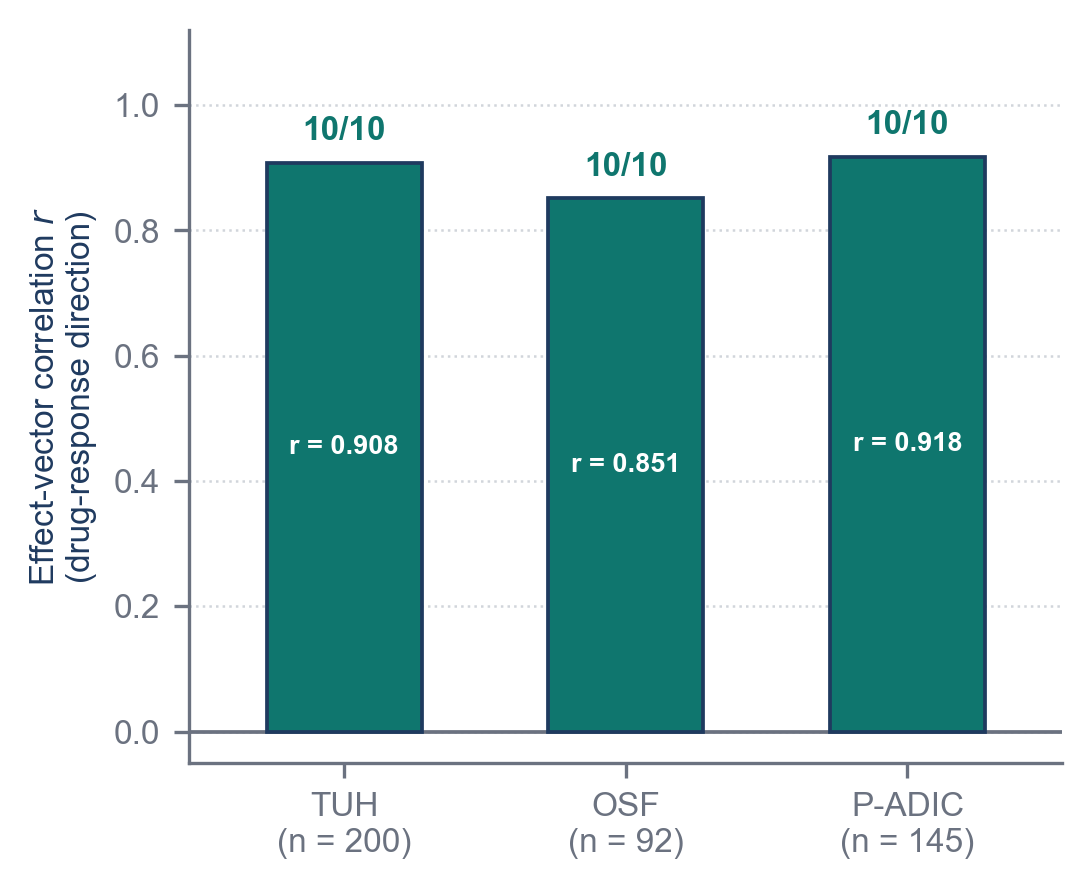
\includegraphics[width=\columnwidth]{figures/fig2_direction_agreement.png}
\caption{Locked fold-0 seed-42 checkpoint only: external signature concordance scored against the training constrained signature. Bars show full-sample effect-vector correlation $r$ for TUH ($r{=}0.908$, $n{=}200$), OSF ($r{=}0.851$, $n{=}92$), and P-ADIC ($r{=}0.918$, $n{=}145$). These bars are not representative of five-fold or multi-seed performance. Secondary signed agreement was 10/10 on each cohort. These values are checkpoint-specific signature concordance, not independent pharmacodynamic validation.}
\label{fig:direction}
\end{figure}
Subject-bootstrap 95\% percentile intervals were 0.874-0.900, 0.790-0.837, and 0.871-0.904. Five-fold means were \(0.385\pm0.308\), \(0.371\pm0.294\), and \(0.372\pm0.310\); signs were 10/10 on three folds, 9/10 on fold 4, and 8/10 on fold 2. Holding folds fixed and varying train seeds \(\{42,7,21,123,2024\}\), non-42 continuous \(r\) typically ranged 0.08-0.43 while signs remained mostly 9/10-10/10 (Table~\ref{tab:multiseed-direction}).
% Table 6 -- Fixed-fold multi-seed training sensitivity (READ-ONLY from aggregate_results)
\begin{table}[!t]
\centering
\caption{Fixed-fold training-seed sensitivity of external direction metrics.
Fold assignment and fold-0 subject membership were frozen at \texttt{split\_seed}${}={}$42;
only \texttt{train\_seed} varied. Seed 42 is the locked historical checkpoint
(\texttt{checkpoint\_constrained.pt}); seeds 7, 21, 123, and 2024 are independent
training-seed perturbations under the same fold split. Values are Pearson $r$
(mean Donepezil/Memantine effect-vector correlation) and sign agreement.
Source: \texttt{models/validation/multiseed\_robustness/aggregate\_results.csv}.}
\label{tab:multiseed-direction}
\setlength{\tabcolsep}{3.5pt}
\begin{tabular}{@{}rlccc@{}}
\toprule
Seed & Role & TUH ($r$; agree) & OSF ($r$; agree) & P-ADIC ($r$; agree) \\
\midrule
42 & Locked fold-0 & 0.908; 10/10 & 0.851; 10/10 & 0.918; 10/10 \\
7 & Alternate train seed & 0.408; 10/10 & 0.408; 10/10 & 0.428; 10/10 \\
21 & Alternate train seed & 0.154; 10/10 & 0.160; 10/10 & 0.106; 8/10 \\
123 & Alternate train seed & 0.147; 9/10 & 0.230; 9/10 & 0.080; 9/10 \\
2024 & Alternate train seed & 0.163; 10/10 & 0.182; 10/10 & 0.146; 10/10 \\
\midrule
\multicolumn{2}{@{}l}{Mean $r$ (all five)} & 0.356 & 0.366 & 0.336 \\
\multicolumn{2}{@{}l}{Median $r$} & 0.163 & 0.230 & 0.146 \\
\multicolumn{2}{@{}l}{SD $r$} & 0.328 & 0.288 & 0.354 \\
\bottomrule
\end{tabular}
\end{table}

Constrained signs exceeded unconstrained signs in all 15 seed\(\times\)cohort cells without establishing continuous-\(r\) stabilization. An equal-weight fold ensemble (\(r=0.642/0.626/0.627\)) did not clearly exceed prior-only mean \(r=0.636\). Under SEME, signed concordance is the more reproducible external component; locked high \(r\) is not architecture-level.

\subsection{Magnitude escalation}

Magnitude \(\bar{s}\) was tested in sequence (Table~\ref{tab:diagnostic-results}; Fig.~\ref{fig:diagnostic}).
% Table 3 -- Diagnostic magnitude discrimination (all contrasts)
% Caption ABOVE tabular (Elsevier). Requires booktabs, adjustbox.
\begin{table*}[!t]
\centering
\footnotesize
\setlength{\tabcolsep}{3.5pt}
\caption{Twin latent drug-response magnitude discrimination across escalating
external cohorts. Status strings are taken from the validation JSON
(\texttt{FAIL}, \texttt{PASS\_WITH\_CAVEATS}). The OSF primary row uses
\texttt{honest\_verdict.status}; OSF disease-label sensitivity rows have no
status field (shown as --). The Kruskal--Wallis row reports $H$ instead of
Cohen's $d$ and Kruskal $p$ in the $p$ column.}
\label{tab:diagnostic-results}
\begin{adjustbox}{max width=\textwidth}
\begin{tabular}{@{}llp{3.6cm}lll@{}}
\toprule
Dataset & Contrast & N (A / B) & $p$ & $d$ & Status \\
\midrule
  \multicolumn{6}{@{}l@{}}{\textbf{TUH}} \\
  \midrule
  TUH & Abnormal vs normal & 131 / 69 & $0.272$ & -0.13 & FAIL \\
  \multicolumn{6}{@{}l@{}}{\textbf{OSF}} \\
  \midrule
  OSF & AD vs HC & 80 / 12 & $p{<}0.001$ & 0.44 & PASS$^{\ast}$ \\
  OSF & AD vs HC (disease${=}0$) & 80 / 12 & $p{<}0.001$ & 0.64 & -- \\
  OSF & AD vs HC (disease${=}1$) & 80 / 12 & $p{<}0.001$ & 0.34 & -- \\
  \multicolumn{6}{@{}l@{}}{\textbf{P-ADIC}} \\
  \midrule
  P-ADIC & AD vs HC & 49 / 96 & $0.968$ & -0.07 & FAIL \\
  P-ADIC & AD vs HC (disease${=}0$) & 49 / 96 & $0.527$ & -0.16 & FAIL \\
  P-ADIC & AD vs HC (disease${=}1$) & 49 / 96 & $0.702$ & -0.14 & FAIL \\
  \multicolumn{6}{@{}l@{}}{\textbf{CAUEEG}} \\
  \midrule
  CAUEEG & Dementia vs Normal & 291 / 436 & $0.516$ & -0.00 & FAIL \\
  CAUEEG & Dementia vs MCI & 291 / 395 & $0.877$ & 0.07 & FAIL \\
  CAUEEG & MCI vs Normal & 395 / 436 & $0.363$ & -0.07 & FAIL \\
  CAUEEG & AD-tagged Dem.\ vs Normal & 214 / 436 & $0.624$ & -0.01 & FAIL \\
  CAUEEG & Kruskal--Wallis (3 groups) & 436 / 395 / 291 & $0.637$ & $H{=}0.90$ & FAIL \\
  CAUEEG & Dem.\ vs Normal (disease${=}0$) & 291 / 436 & $0.411$ & -0.04 & FAIL \\
  CAUEEG & Dem.\ vs Normal (disease${=}1$) & 291 / 436 & $0.776$ & 0.00 & FAIL \\
\bottomrule
\end{tabular}
\end{adjustbox}
\vspace{0.3em}\\
{\scriptsize $^{\ast}$\texttt{PASS\_WITH\_CAVEATS} (HC $n{=}12$; exploratory).}
\end{table*}

\begin{figure*}[!t]
\centering
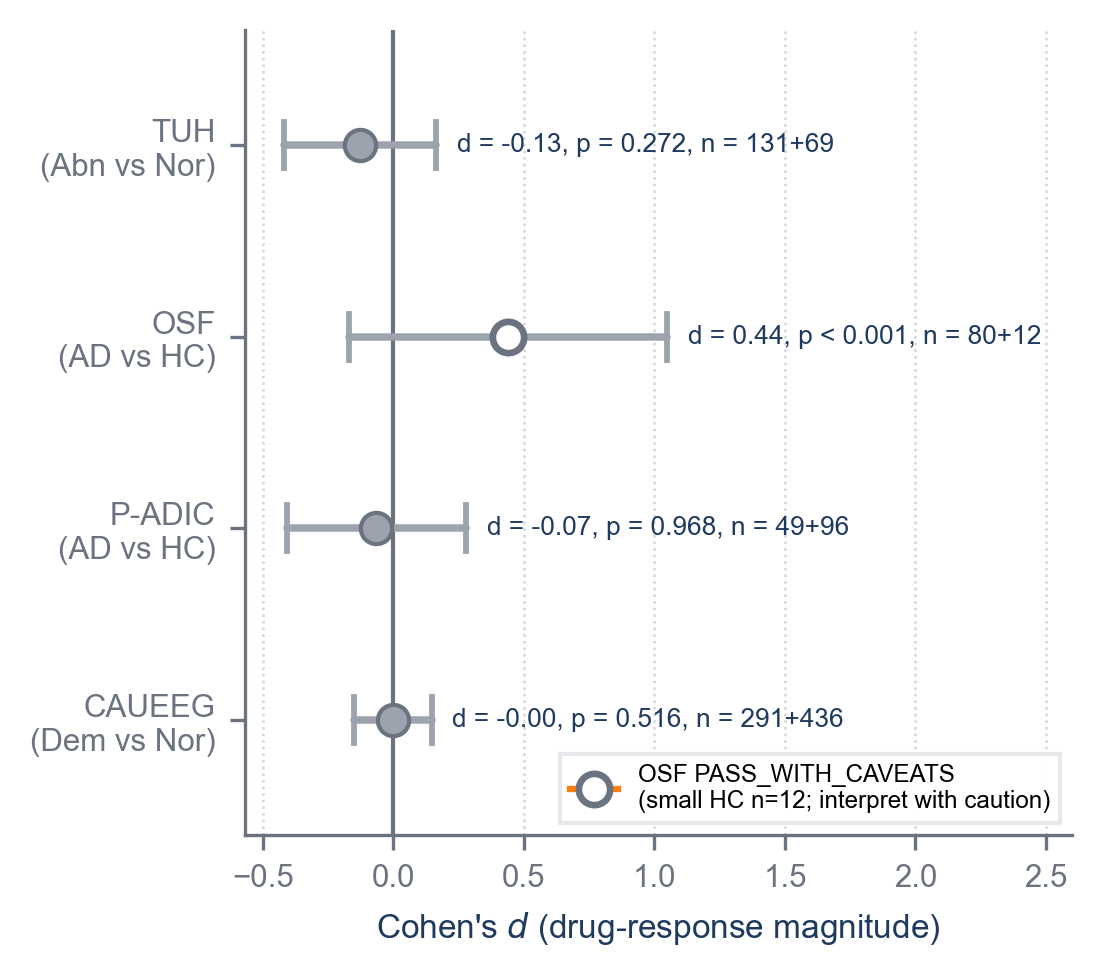
\includegraphics[width=0.92\textwidth]{figures/fig3_diagnostic_null.png}
\caption{Forest plot of Cohen's $d$ for primary twin magnitude contrasts on TUH, OSF, P-ADIC, and CAUEEG. Approximate 95\% intervals use the Hedges--Olkin standard-error formula from reported $d$ and group sizes. Exact $n$, $p$, and $d$ values are listed in Table~\ref{tab:diagnostic-results}.}
\label{fig:diagnostic}
\end{figure*}
 TUH abnormal versus normal was null (p = 0.272, d = -0.13). OSF AD versus HC was an exploratory positive with HC \(n=12\) caveats (p = 0.000278, d = 0.44). P-ADIC AD versus HC was null (p = 0.968, d = -0.07). CAUEEG Dementia versus Normal was null (p = 0.516, d = 0.00, \(n=727\)), despite clear theta/alpha slowing on the same features (p < 0.001, d = 0.47) and good scale/PCA overlap (Fig.~\ref{fig:pca}).
\begin{figure}[!t]
\centering
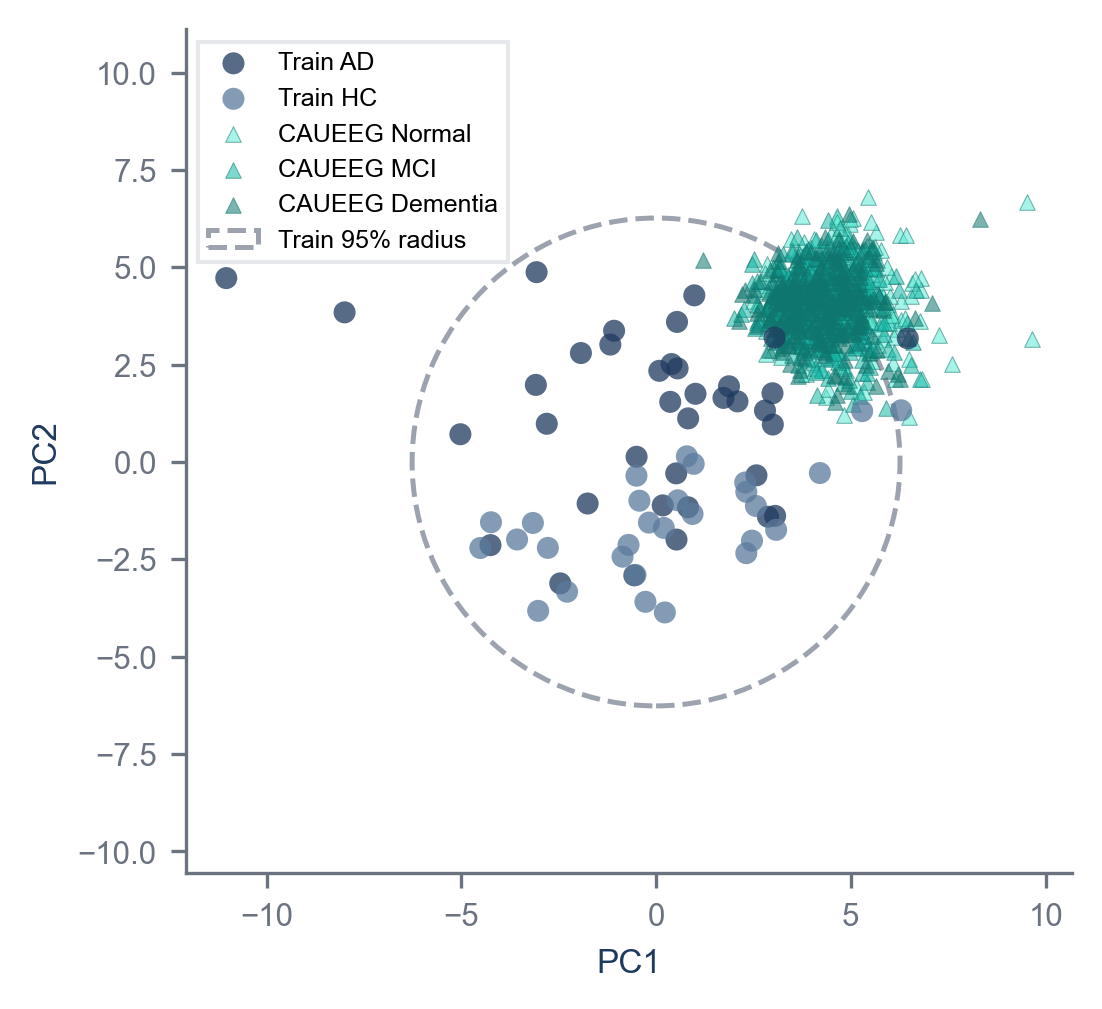
\includegraphics[width=\columnwidth]{figures/fig4_pca.png}
\caption{PCA of 2185-D features: training cohort versus CAUEEG. Dashed circle marks the training 95\% radius; overlap fraction within that radius is 0.611.}
\label{fig:pca}
\end{figure}
Secondary CAUEEG contrasts and disease-label ablations remained null. Magnitude does not provide reliable external diagnosis in this escalation.

\subsection{Encoding bake-off (classical features versus latent)}

On CAUEEG Dementia versus Normal (\(n=727\)), SEME's Encoding axis compares classical feature references to frozen-twin \(\mu_{\mathrm{base}}\) readouts (Fig.~\ref{fig:encoding}; Fig.~\ref{fig:bakeoff}; Table~\ref{tab:encoding-results}). A logistic probe on \(\mu_{\mathrm{base}}\) (disease bit fixed to 0) reached mean ROC-AUC 0.579 (permutation p = 0.010). Theta/alpha reached 0.675 (OOF 0.673) and a packed 2185-D logistic reference reached 0.699 (OOF 0.699; feature-space reference, not a CVAE score). Nested heads peaked at OOF AUC 0.593 (permutation p = 0.005); MLP and boosting did not close the gap.
\begin{figure*}[!t]
\centering
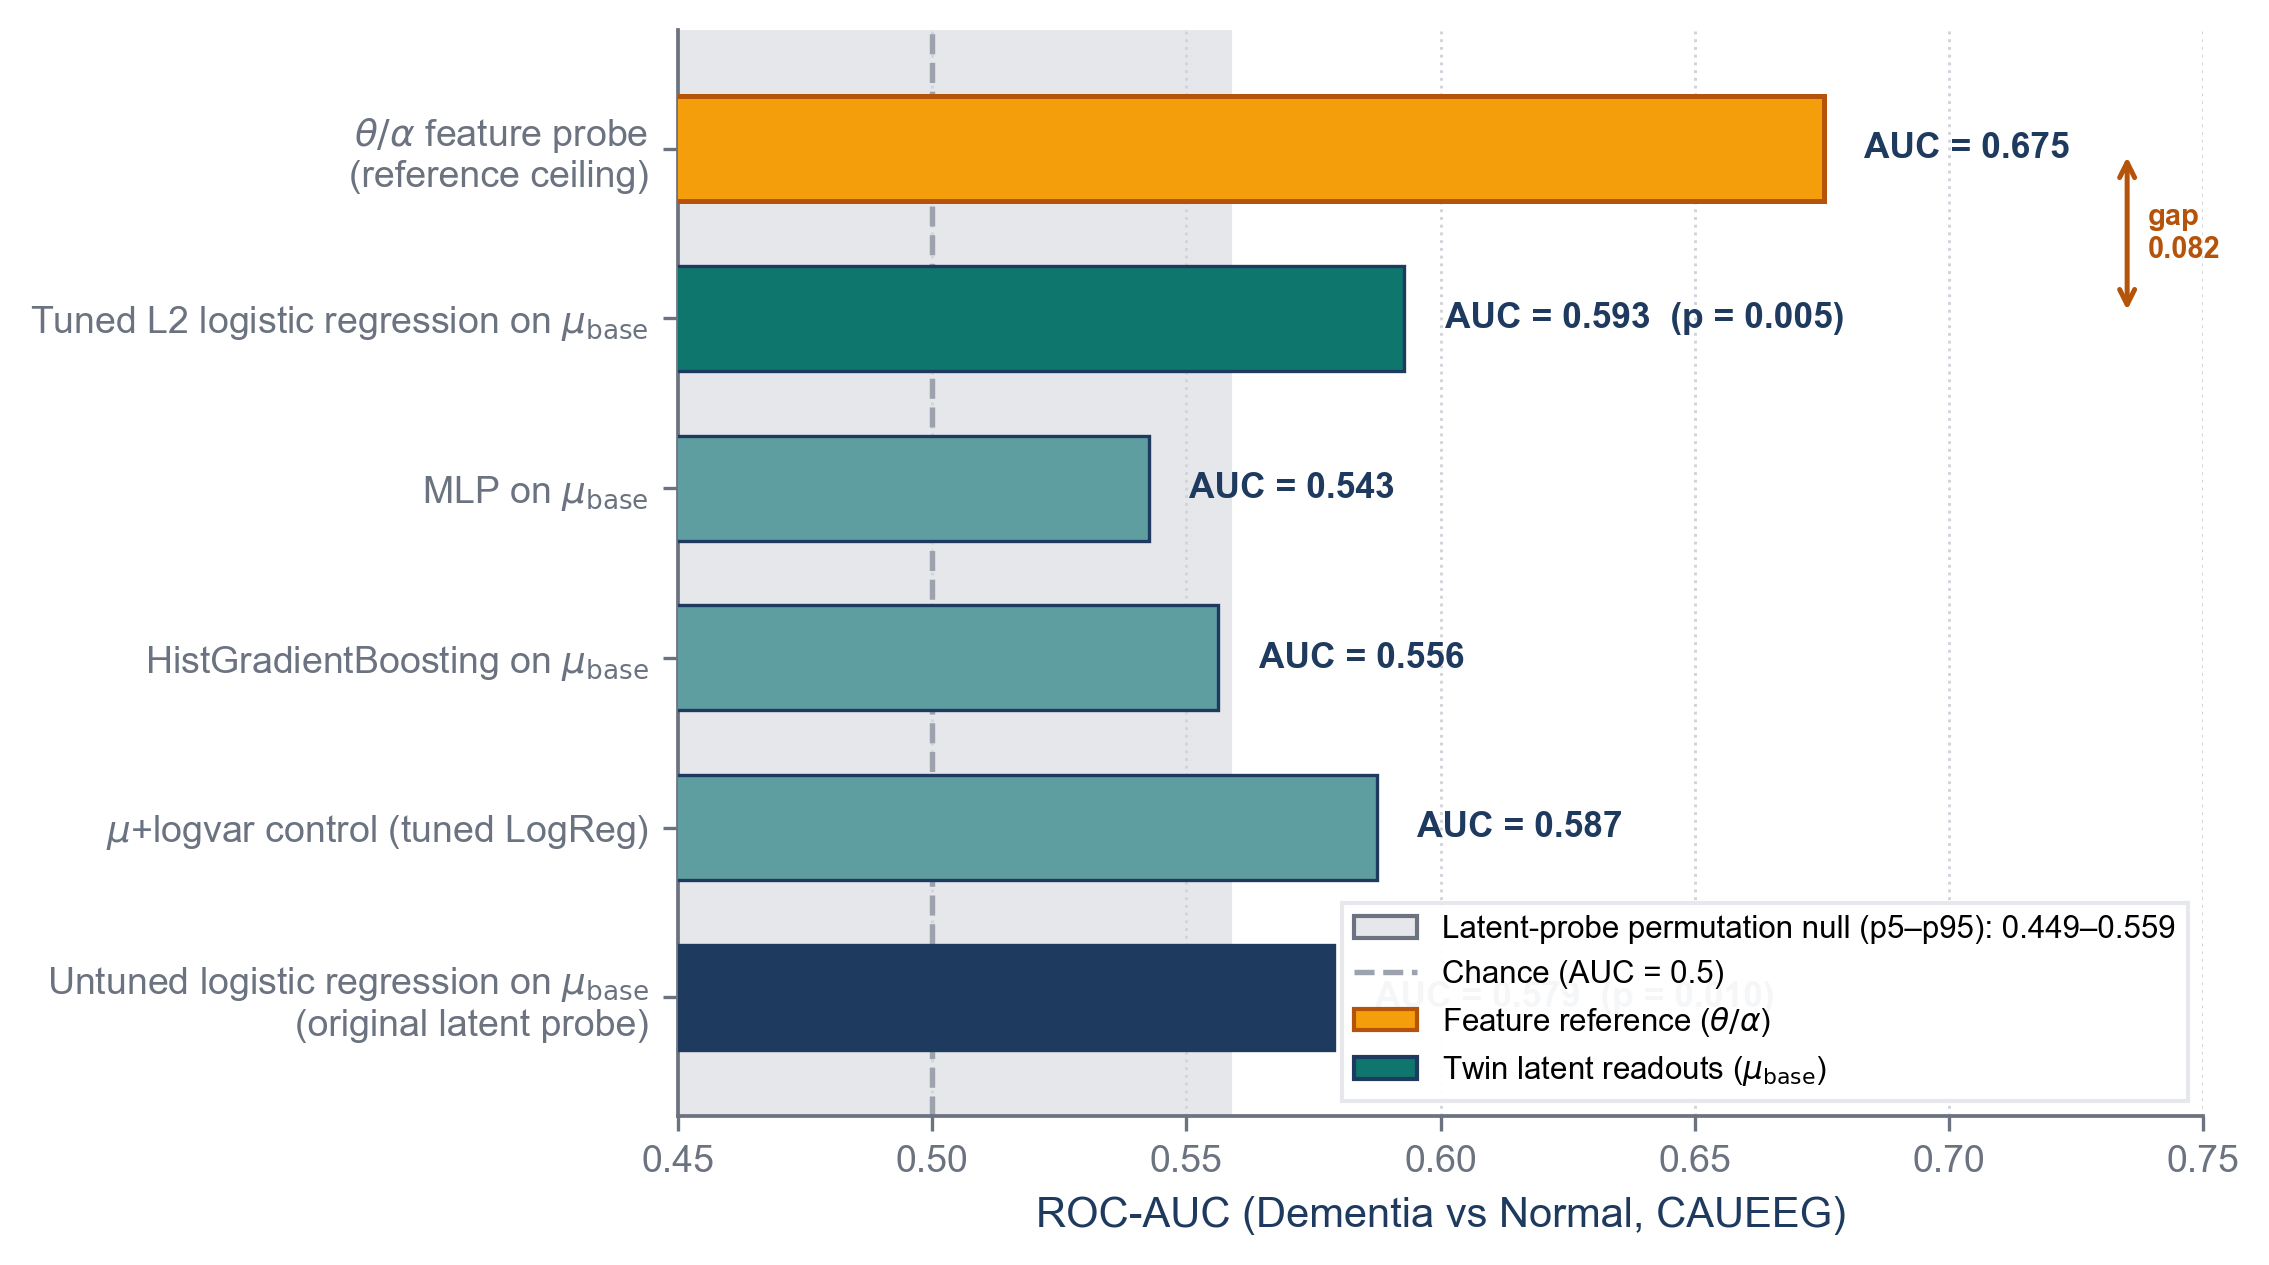
\includegraphics[width=0.95\textwidth]{figures/fig5_encoding_analysis.png}
\caption{SEME Encoding bake-off on CAUEEG Dementia versus Normal ($n{=}727$). Amber: classical theta/alpha and related feature references. Teal/navy: frozen-twin $\mu_{\mathrm{base}}$ readouts. Gray band: latent-probe permutation null 5th--95th percentiles (0.449--0.559). Best nested head OOF AUC $= 0.593$. A packed 2185-D logistic feature-space reference reaches mean-fold AUC $= 0.699$ (not a CVAE score).}
\label{fig:encoding}
\end{figure*}
% Table 4 -- Encoding analysis (pairs with Fig. 5)
% Caption ABOVE tabular. Requires booktabs, adjustbox.
\begin{table}[!t]
\centering
\footnotesize
\setlength{\tabcolsep}{3pt}
\caption{CAUEEG Dementia vs Normal encoding analysis ($n = 727$).
Out-of-fold (OOF) ROC-AUC and balanced accuracy are reported.
Permutation $p$-values are included where computed (original latent probe:
200 label shuffles of 5-fold CV; best head: 200 shuffles of nested CV).
The 2185-D logistic row is a raw feature-space diagnostic reference, not a CVAE result,
not a theoretical upper bound, and not a supervised deep 2185-D classifier. The final column is OOF AUC minus the $\theta/\alpha$
pooled OOF AUC ($0.673$; mean-fold $\theta/\alpha$ AUC $= 0.675$ is used in the prose
and Fig.~\ref{fig:encoding}). Complements Fig.~\ref{fig:encoding}.}
\label{tab:encoding-results}
\begin{adjustbox}{max width=\columnwidth}
\begin{tabular}{@{}lccccc@{}}
\toprule
Model & Input & AUC & Bal.\ acc. & Perm.\ $p$ & vs.\ $\theta/\alpha$ \\
\midrule
  2185-D logistic (feature ref.) & packed 2185-D & 0.699 & 0.642 & -- & +0.026 \\
  $\theta/\alpha$ probe (ref.) & $\theta/\alpha$ & 0.673 & 0.625 & -- & +0.000 \\
  Untuned logistic & $\mu_{\mathrm{base}}$ & 0.576 & 0.568 & $0.010$ & -0.097 \\
  Tuned L2 logistic & $\mu_{\mathrm{base}}$ & 0.593 & 0.573 & $0.005$ & -0.080 \\
  MLP & $\mu_{\mathrm{base}}$ & 0.543 & 0.543 & -- & -0.130 \\
  HistGradientBoosting & $\mu_{\mathrm{base}}$ & 0.556 & 0.548 & -- & -0.117 \\
  Tuned LogReg ($\mu$+logvar) & $\mu$+logvar & 0.587 & 0.554 & -- & -0.085 \\
\bottomrule
\end{tabular}
\end{adjustbox}
\end{table}

\begin{figure}[!t]
\centering
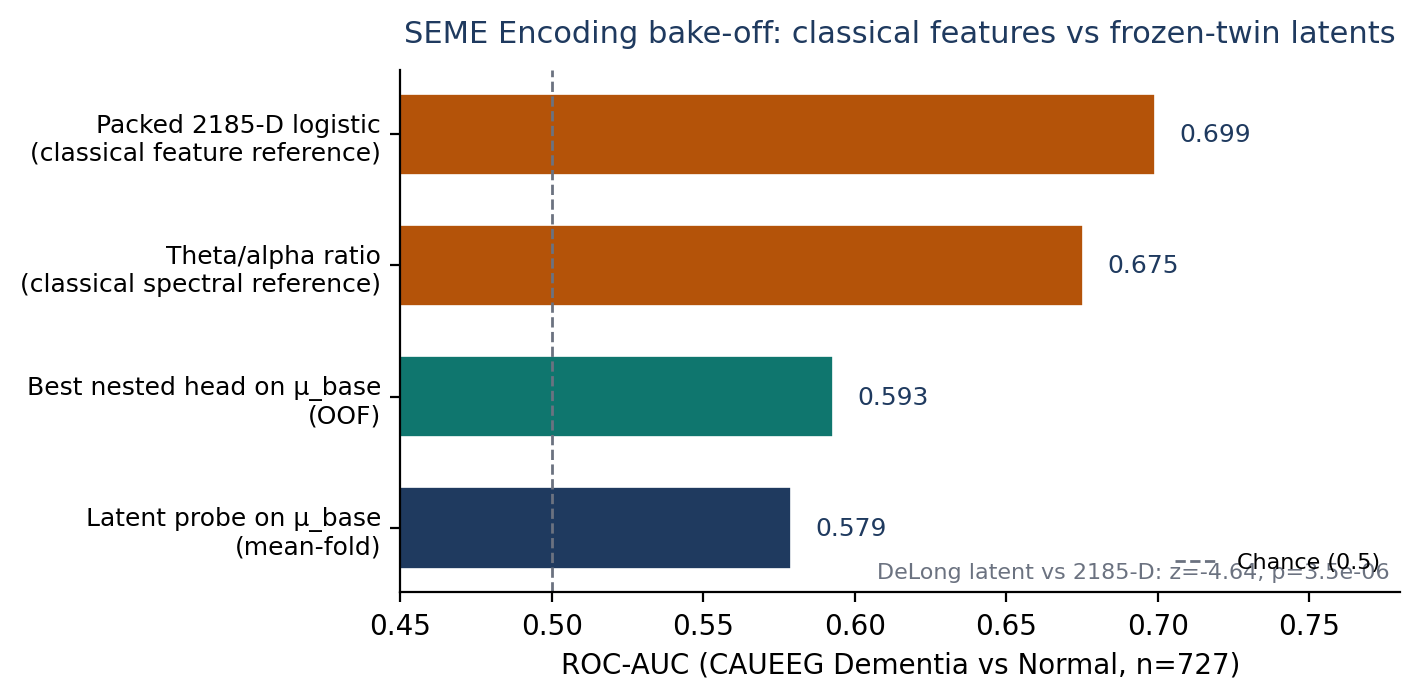
\includegraphics[width=\columnwidth]{figures/fig_bakeoff_encoding.png}
\caption{Compact SEME Encoding bake-off panel: classical feature references versus latent/head readouts on CAUEEG Dementia versus Normal ($n{=}727$). Values match locked probe/head artifacts; DeLong annotation uses the non-locked Phase~C OOF comparison when available.}
\label{fig:bakeoff}
\end{figure}
Paired DeLong tests confirmed latent below theta/alpha (z = -3.63, p = 0.000285) and below 2185-D (z = -4.64, p $<$ 0.001), and best head below both references (z = -3.32 and -4.09; p $<$ 0.001); theta/alpha versus 2185-D was not significant (z = -1.11, p = 0.268). Unconstrained latent AUC (0.539) did not exceed constrained (0.579). The bake-off shows encoding-level attenuation under tested readouts, not an information-bottleneck proof.

\subsection{Constraint-weight sweep}

An exploratory fold-0 \(\alpha_c\) sweep (Fig.~\ref{fig:alpha}) showed signs at 10/10 by \(\alpha_c=0.05\), TUH \(r\) peaking near \(\alpha_c=0.1\) (\(r=0.897\)), and non-monotone latent AUC. It does not support a simple direction-versus-diagnosis trade-off and is not a nested \(\alpha_c\) selection.

\begin{figure}[!t]
\centering
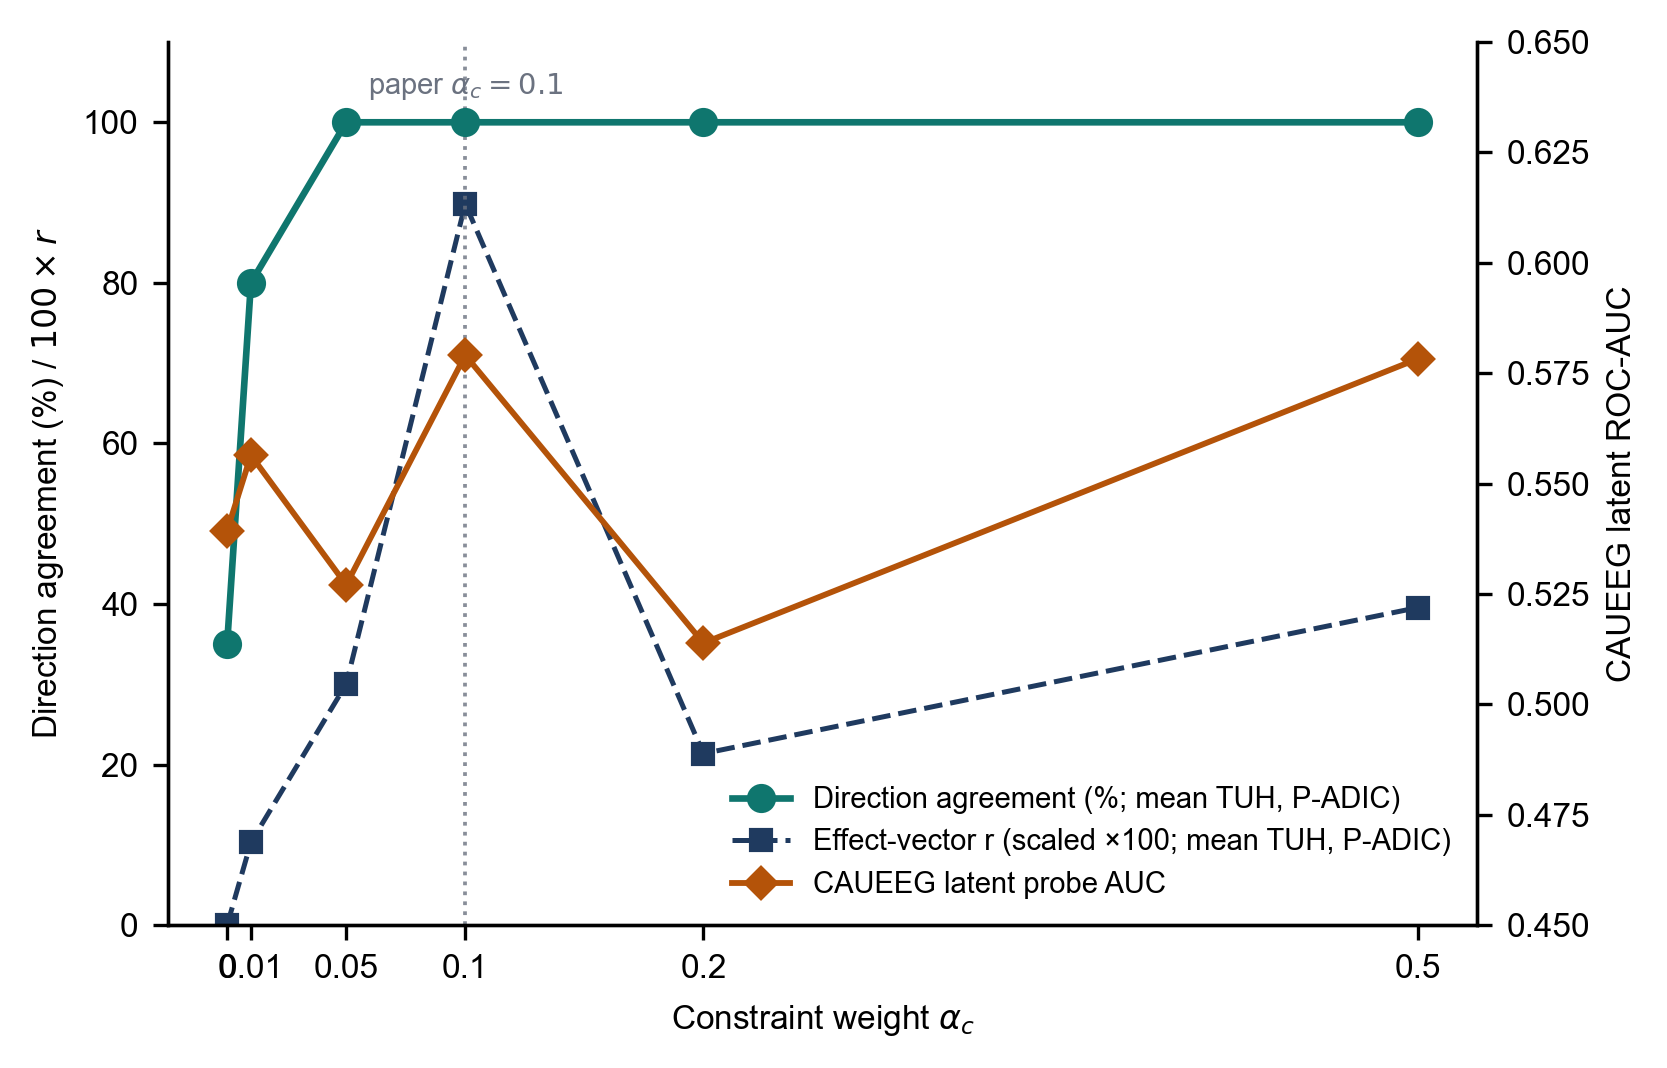
\includegraphics[width=\columnwidth]{figures/fig6_constraint_strength.png}
\caption{Exploratory fold-0 constraint-weight ($\alpha_c$) sweep: signed direction agreement and continuous effect-vector correlation, with CAUEEG latent-probe AUC. Not a nested selection of $\alpha_c$.}
\label{fig:alpha}
\end{figure}

\subsection{ChemBERTa versus padded one-hot}

A matched fold-0 constrained retrain replaced ChemBERTa with 384-D padded one-hot drug IDs without touching the locked checkpoint. One-hot reached 10/10 signs on TUH/OSF/P-ADIC (\(r=0.176/0.194/0.174\)); rematched ChemBERTa reached 9/10 (\(r=0.104/0.110/0.076\)). Both continuous-\(r\) values sit in the low multi-seed regime. CAUEEG latent mean AUC was 0.540 (ChemBERTa rematch) versus 0.559 (one-hot). In this two-drug setting, chemical embeddings are not required for constraint-consistent signs; the locked ChemBERTa twin remains the primary historical checkpoint.


\section{Discussion}
\label{sec:discussion}
\input{sections/06_discussion}

\section{Conclusion}
\label{sec:conclusion}
\input{sections/07_conclusion}

\section*{CRediT authorship contribution statement}

Author contributions will be completed when the author list is finalized. No corresponding author is designated in this draft.



\subsection{Ethics statement}

This work is a secondary analysis of de-identified EEG datasets. No new human participants were recruited and no clinical interventions were performed. Training resting-state EEG features derive from the public OpenNeuro accession ds004504 (Miltiadous et al.). External cohorts were obtained under each provider's academic data-use terms: the Temple University Hospital (TUH) EEG Corpus data use agreement; a public Open Science Framework (OSF) Eyes\_closed AD/HC partition; the Dryad P-ADIC release (DOI 10.5061/dryad.8gtht76pw); and academic, non-commercial access to CAUEEG granted by the CAUEEG team (access contact: Min-jae Kim), with no redistribution of raw CAUEEG or TUH recordings. Analyses were conducted for academic research. The study does not claim prospective clinical decision support.



\subsection{Funding}

This research received no specific grant from funding agencies in the public, commercial, or not-for-profit sectors.



\section*{Data availability}

Training resting-state EEG features used in this project are from OpenNeuro accession ds004504 (Miltiadous et al. AD/HC resting EEG), processed to the feature arrays described in Methods. Temple University Hospital (TUH) clinical EEG is available to researchers under the TUH corpus data use agreement and cannot be redistributed by the authors. The OSF Eyes\_closed AD/HC features used for the AD/HC external magnitude and direction checks were imported from a public OSF-hosted partition already present in the project archive. P-ADIC AD and control matrices are available from Dryad (DOI 10.5061/dryad.8gtht76pw) under the release terms of Shor et al. CAUEEG raw recordings were obtained by academic application to the CAUEEG team (access granted by Min-jae Kim; Kim et al., NeuroImage 2023) for non-commercial research use and must not be redistributed. Derived project artifacts that can be shared subject to those upstream terms include processed feature arrays generated in this repository (where redistribution is allowed), validation JSON summaries, and analysis code. Raw CAUEEG and TUH EDFs will not be redistributed by the authors. File-level paths are listed in Supplementary Material S1.



\subsection{Code availability}

Analysis and figure-generation code for this manuscript live in the local project repository and are not currently in a public repository. The Python environment is the project virtualenv \texttt{eeg\_twin} (Python 3.10); install from \texttt{requirements.\allowbreak{}txt} into that environment. Exact script names, configuration keys, checkpoint aliases, and regeneration commands are listed in Supplementary Material S1 and \texttt{paper/\allowbreak{}CODE\_\allowbreak{}AVAILABILITY.\allowbreak{}md}. A public mirror (URL and commit hash) will be linked at acceptance; until then, the packaged Overleaf zip and the local repository are the reproducibility sources for the reported JSON and figures.



\section*{Glossary}

Terms below follow Methods and Results. They do not introduce new endpoints or claims.


\begin{itemize}
  \item \textbf{CVAE:} conditional variational autoencoder.
  \item \textbf{EEG:} electroencephalography.
  \item \textbf{PD:} pharmacodynamic. In this paper the label names the literature-prior training objective, not empirical post-dose pharmacodynamic validation.
  \item \textbf{ROC-AUC:} area under the receiver operating characteristic curve.
  \item \textbf{OOF:} out-of-fold.
  \item \textbf{TUH:} Temple University Hospital EEG corpus.
  \item \textbf{OSF:} Open Science Framework Eyes\_closed AD/HC set used here.
  \item \textbf{CAUEEG:} Chung-Ang University Hospital EEG dataset.
  \item \textbf{P-ADIC:} p-adic quantum potential EEG cohort (Shor et al.; Dryad).
  \item \textbf{ChemBERTa:} chemical Bidirectional Encoder Representations from Transformers. Here, frozen precomputed embeddings for Donepezil and Memantine, not a large-library chemistry test.
  \item \textbf{MSE:} mean squared error (reconstruction term).
  \item \textbf{KL:} Kullback-Leibler divergence (CVAE regularizer).
  \item \textbf{ICA:} independent component analysis (FastICA on the training path).
  \item \textbf{FIR:} finite impulse response filter (training band-pass 0.5-40 Hz).
  \item \textbf{PCA:} principal component analysis.
  \item \textbf{Latent representation:} CVAE latent mean under specified conditioning (baseline: zero-drug). Residual diagnostic content is scored with probes, not as an information-theoretic bottleneck.
  \item \textbf{Drug-response signature:} the training constrained signature (mean simulated drug-minus-baseline feature vector). External direction scoring is concordance with that signature, not post-dose pharmacodynamic validation.
  \item \textbf{Digital twin:} the constrained CVAE used for in silico EEG-drug signature simulation. It is not a clinically validated pharmacodynamic model.
  \item \textbf{Effect vector:} cohort-mean drug-minus-baseline feature vector used to compute Pearson r and block-level sign agreement.
\end{itemize}


\section*{Declaration of competing interests}

The authors declare that they have no known competing financial interests or personal relationships that could have appeared to influence the work reported in this paper.



\section*{Acknowledgments}

We thank the Temple University Hospital (TUH) EEG Corpus team for access to clinical EEG under the TUH data use agreement; Min-jae Kim and the CAUEEG investigators for academic access to the Chung-Ang University Hospital EEG dataset; and the providers of OpenNeuro ds004504 (Miltiadous et al.), the OSF Eyes\_closed AD/HC partition, and the Dryad P-ADIC release. We also thank the Alzheimer's Disease Neuroimaging Initiative (ADNI) for related clinical data infrastructure used in supporting cohort work outside the primary EEG external battery.


\appendix
\renewcommand{\thetable}{A.\arabic{table}}
\renewcommand{\thefigure}{A.\arabic{figure}}
\renewcommand{\theHtable}{A.\arabic{table}}
\renewcommand{\theHfigure}{A.\arabic{figure}}
\setcounter{table}{0}
\setcounter{figure}{0}
\section{Reproducibility appendix}
\label{sec:supp-repro}
This appendix lists configuration keys, scripts, and artifact paths used to regenerate the manuscript numbers. It is not required to follow the scientific argument in the main text. Table~\ref{tab:reviewer-defense} lists methodological safeguards and remaining scope boundaries, including non-locked Phase~C DeLong and ChemBERTa-versus-one-hot rows.


\subsection{Reproduction contract}

\begin{itemize}
  \item Environment: Python 3.10.0 in \texttt{eeg\_twin/}; PyTorch 2.10.0+cu128; NumPy 1.26.4; SciPy 1.15.3; scikit-learn 1.7.2; MNE 1.11.0; Transformers 5.0.0 (\texttt{computational\_\allowbreak{}requirements.\allowbreak{}json}).
  \item Hardware: NVIDIA GeForce RTX 5060 Ti (16 GB).
  \item Split: subject-level \texttt{StratifiedKFold} (\texttt{n\_splits=5}, \texttt{random\_\allowbreak{}state=42}); within-fold validation \texttt{random\_\allowbreak{}state=42+fold\_\allowbreak{}idx}.
  \item Locked checkpoint: \texttt{models/\allowbreak{}checkpoints\_\allowbreak{}constrained/\allowbreak{}checkpoint\_\allowbreak{}constrained.\allowbreak{}pt} = \texttt{fold\_\allowbreak{}0\_\allowbreak{}best.\allowbreak{}pt}, epoch 99, \texttt{constraint\_\allowbreak{}weight=0.\allowbreak{}1}, selection = minimum fold-0 validation total loss (0.0241).
  \item Matched unconstrained: \texttt{models/\allowbreak{}checkpoints\_\allowbreak{}unconstrained/\allowbreak{}checkpoint\_\allowbreak{}unconstrained.\allowbreak{}pt} from \texttt{checkpoints\_\allowbreak{}5fold/\allowbreak{}fold\_\allowbreak{}0\_\allowbreak{}best.\allowbreak{}pt}.
  \item Variant: \texttt{constrained\_\allowbreak{}mlp}; 2,648,777 trainable parameters; ChemBERTa embeddings frozen \texttt{.npy} files.
  \item Preprocessing: FIR 0.5--40 Hz, training notch 50 Hz, FastICA with empty default exclusion, 4 s epochs at 90\% overlap, per-subject z-score after epoching, Welch \texttt{n\_\allowbreak{}per\_\allowbreak{}seg=256} at 500 Hz.
  \item Feature map: 2185-D, 0-based slices PSD \texttt{[0,380)}, bands \texttt{[380,475)}, interleaved connectivity \texttt{[475,2185)}; \(L_{\mathrm{conn}}\) window \texttt{[475,1330)}.
  \item Dummy-batch inference (not clinical real-time or end-to-end latency): 0.602 ms/subject; dummy throughput 1660 subjects/s; peak dummy-forward GPU memory 50.2 MiB; checkpoint 31,876,749 bytes. Training wall-clock for the locked run is not logged.
  \item Expected locked direction outputs (fold-0 seed-42): \(r = 0.908 / 0.851 / 0.918\) and 10/10 signs on TUH / OSF / P-ADIC against the training constrained signature.
  \item Master roll-up: \texttt{models/\allowbreak{}validation/\allowbreak{}complete\_\allowbreak{}validation\_\allowbreak{}report\_\allowbreak{}v3.\allowbreak{}json}.
\end{itemize}

\subsection{Model configuration}

\begin{itemize}
  \item Variant: \texttt{constrained\_\allowbreak{}mlp} in \texttt{src/\allowbreak{}models/\allowbreak{}config.\allowbreak{}py} (\texttt{MODEL\_\allowbreak{}VARIANTS['constrained\_\allowbreak{}mlp']}).
  \item ChemBERTa input dim: \texttt{MODEL\_\allowbreak{}CONFIG['drug\_\allowbreak{}encoder']['input\_\allowbreak{}dim'] = 384}.
  \item CVAE latent dim: \texttt{MODEL\_\allowbreak{}CONFIG['cvae']['latent\_\allowbreak{}dim'] = 128}.
  \item Hidden widths: EEG encoder [256, 512], drug encoder [256, 128], CVAE [512, 256]; \texttt{use\_\allowbreak{}attention: False}.
  \item KL weight: \texttt{TRAINING\_\allowbreak{}CONFIG['beta\_\allowbreak{}kl'] = 0.\allowbreak{}01}.
  \item Constraint schedule: \texttt{warmup\_\allowbreak{}epochs = 5}, paper \texttt{constraint\_\allowbreak{}weight = 0.\allowbreak{}1} in \texttt{run\_\allowbreak{}constrained\_\allowbreak{}training.\allowbreak{}py}. Implemented \(\alpha_c(t)=\alpha_c^{\star}\min(1,(t-T_w)/5)\) for \(t\ge T_w\) with 0-indexed \(t\), so \(\alpha_c(T_w)=0\).
  \item Parameter count: 2,648,777 (\texttt{models/\allowbreak{}validation/\allowbreak{}computational\_\allowbreak{}requirements.\allowbreak{}json}).
  \item Fold-0 loss histories: \texttt{models/\allowbreak{}evaluation/\allowbreak{}constrained\_\allowbreak{}evaluation\_\allowbreak{}report.\allowbreak{}json} → \texttt{constraint\_\allowbreak{}curves.\allowbreak{}fold\_\allowbreak{}0} (Fig.~\ref{fig:traincurves}).
\end{itemize}

\subsection{Pharmacodynamic priors and loss helpers}

\begin{itemize}
  \item Priors store: \texttt{src/\allowbreak{}drugs/\allowbreak{}pharmacological\_\allowbreak{}embedding.\allowbreak{}py} (\texttt{DRUG\_\allowbreak{}PHARMACOLOGY[*]['eeg\_\allowbreak{}effects']}).
  \item Prior loader: \texttt{get\_\allowbreak{}eeg\_\allowbreak{}effect\_\allowbreak{}prior(drug\_\allowbreak{}name)}.
  \item Band constraint: \texttt{compute\_\allowbreak{}band\_\allowbreak{}direction\_\allowbreak{}constraint} in \texttt{src/\allowbreak{}models/\allowbreak{}losses.\allowbreak{}py}.
  \item Connectivity constraint: \texttt{compute\_\allowbreak{}connectivity\_\allowbreak{}constraint}.
  \item Band / connectivity index slices used by external direction scoring: \texttt{BAND\_SLICES} in \texttt{src/\allowbreak{}tuh/\allowbreak{}tuh\_\allowbreak{}validation.\allowbreak{}py} (delta [380:399], theta [399:418], alpha [418:437], beta [437:456], connectivity [475:1330]).
  \item Flatten order (\texttt{api/\allowbreak{}utils/\allowbreak{}feature\_\allowbreak{}processor.\allowbreak{}py} \texttt{flatten\_\allowbreak{}features}): PSD [0:380), band powers [380:475), then for each of five bands coherence upper-triangle (171) then PLV (171), so full connectivity is interleaved on [475:2185). Coherence and PLV are \textbf{not} contiguous pure blocks. The training connectivity constraint and direction-scoring window \texttt{[475:1330)} match \texttt{CONNECTIVITY\_\allowbreak{}INDICES} / \texttt{BAND\_\allowbreak{}SLICES['connectivity']}; that window mixes interleaved coh/PLV from early bands and must not be cited as an all-coherence block. Do not use \texttt{feature\_\allowbreak{}block\_\allowbreak{}ranges()['coherence\_\allowbreak{}block']} as a pure-coherence map (it conflicts with interleaving).
\end{itemize}

\subsection{Training data paths and checkpoint aliases}

\begin{itemize}
  \item Training arrays: \texttt{data/\allowbreak{}eeg\_\allowbreak{}features/\allowbreak{}\{AD,HC\}\_\allowbreak{}*.\allowbreak{}npy} (PSD shapes \texttt{(37, 19, 20)} and \texttt{(29, 19, 20)}).
  \item Raw EEGLAB discovery: \texttt{EEGLoader.\allowbreak{}find\_\allowbreak{}eeg\_\allowbreak{}files} under \texttt{data/\allowbreak{}raw\_\allowbreak{}eeg/\allowbreak{}\{AD,HC\}/\allowbreak{}}.
  \item Subject-level CV helper: \texttt{get\_\allowbreak{}subject\_\allowbreak{}level\_\allowbreak{}kfold} (\texttt{n\_\allowbreak{}splits = 5}, \texttt{random\_\allowbreak{}seed = 42} from \texttt{DATA\_CONFIG}).
  \item Constrained evaluation alias: \texttt{models/\allowbreak{}checkpoints\_\allowbreak{}constrained/\allowbreak{}checkpoint\_\allowbreak{}constrained.\allowbreak{}pt} (fold-0 best).
  \item Matched unconstrained alias: \texttt{models/\allowbreak{}checkpoints\_\allowbreak{}unconstrained/\allowbreak{}checkpoint\_\allowbreak{}unconstrained.\allowbreak{}pt} (from \texttt{checkpoints\_\allowbreak{}5fold/\allowbreak{}fold\_\allowbreak{}0\_\allowbreak{}best.\allowbreak{}pt}).
  \item Simulation draws: \texttt{num\_\allowbreak{}samples = 5} in \texttt{simulate\_\allowbreak{}post\_\allowbreak{}drug\_\allowbreak{}eeg} for reported external runs.
\end{itemize}

\subsection{External processing and validation artifacts}

\begin{itemize}
  \item TUH processing: \texttt{process\_\allowbreak{}tuh\_\allowbreak{}eeg.\allowbreak{}py} (\texttt{CROP\_\allowbreak{}SECONDS = 320}, \texttt{TARGET\_\allowbreak{}N\_\allowbreak{}EPOCHS\_\allowbreak{}FOR\_\allowbreak{}PSD = 864}). For locked TUH results, the stored feature provenance in \texttt{data/\allowbreak{}tuh\_\allowbreak{}features/\allowbreak{}processing\_\allowbreak{}report.\allowbreak{}json} records \texttt{crop\_\allowbreak{}seconds=60.\allowbreak{}0} and \texttt{apply\_\allowbreak{}ica=false}; the 320-s value reflects the current script default and was not used to regenerate the locked TUH artifacts.
  \item CAUEEG processing: \texttt{src/\allowbreak{}tuh/\allowbreak{}process\_\allowbreak{}caueeg\_\allowbreak{}eeg.\allowbreak{}py}.
  \item Master report: \texttt{models/\allowbreak{}validation/\allowbreak{}complete\_\allowbreak{}validation\_\allowbreak{}report\_\allowbreak{}v3.\allowbreak{}json}.
  \item Unconstrained battery: \texttt{models/\allowbreak{}validation/\allowbreak{}unconstrained\_\allowbreak{}external\_\allowbreak{}battery.\allowbreak{}json}.
  \item Prior-only baseline: \texttt{models/\allowbreak{}validation/\allowbreak{}prior\_\allowbreak{}only\_\allowbreak{}direction.\allowbreak{}json}.
  \item Fisher-\(z\) CIs for \(r\): \texttt{models/\allowbreak{}validation/\allowbreak{}direction\_\allowbreak{}r\_\allowbreak{}fisher\_\allowbreak{}ci.\allowbreak{}json}.
  \item \(\alpha_c\) sweep: \texttt{models/\allowbreak{}validation/\allowbreak{}constraint\_\allowbreak{}strength\_\allowbreak{}sweep.\allowbreak{}json}.
  \item Latent probe: \texttt{models/\allowbreak{}validation/\allowbreak{}layer5e\_\allowbreak{}caueeg\_\allowbreak{}latent\_\allowbreak{}probe\_\allowbreak{}results.\allowbreak{}json}.
  \item Nested heads: \texttt{models/\allowbreak{}validation/\allowbreak{}layer5e\_\allowbreak{}caueeg\_\allowbreak{}classifier\_\allowbreak{}head\_\allowbreak{}results.\allowbreak{}json}.
\end{itemize}

\subsection{Endpoint implementation notes}

\begin{itemize}
  \item Direction correlation key in JSON: \texttt{effect\_\allowbreak{}magnitude\_\allowbreak{}correlation}.
  \item Subject-bootstrap CIs: \texttt{models/\allowbreak{}validation/\allowbreak{}direction\_\allowbreak{}r\_\allowbreak{}subject\_\allowbreak{}bootstrap\_\allowbreak{}ci.\allowbreak{}json} (B=2000).
  \item Five-fold external direction: \texttt{models/\allowbreak{}validation/\allowbreak{}fold\_\allowbreak{}external\_\allowbreak{}direction\_\allowbreak{}results.\allowbreak{}json}.
  \item Equal-weight fold ensemble: \texttt{models/\allowbreak{}validation/\allowbreak{}fold\_\allowbreak{}ensemble/\allowbreak{}fold\_\allowbreak{}ensemble\_\allowbreak{}external\_\allowbreak{}direction\_\allowbreak{}results.\allowbreak{}json}.
  \item Ensemble subject bootstrap (B=2000, seed 42): \texttt{models/\allowbreak{}validation/\allowbreak{}fold\_\allowbreak{}ensemble/\allowbreak{}bootstrap/\allowbreak{}ensemble\_\allowbreak{}subject\_\allowbreak{}bootstrap\_\allowbreak{}B2000.\allowbreak{}json}.
  \item Prior vs ensemble incremental-value note: \texttt{models/\allowbreak{}validation/\allowbreak{}prior\_\allowbreak{}vs\_\allowbreak{}ensemble/\allowbreak{}} (paired \(\Delta r\) not supportable from stored prior-only artifacts).
  \item Domain-shift LR AUCs (2185-D): \texttt{models/\allowbreak{}validation/\allowbreak{}domain\_\allowbreak{}shift/\allowbreak{}domain\_\allowbreak{}shift\_\allowbreak{}results.\allowbreak{}json}.
  \item Domain-shift forensics (feature families): \texttt{models/\allowbreak{}validation/\allowbreak{}domain\_\allowbreak{}shift\_\allowbreak{}forensics/\allowbreak{}domain\_\allowbreak{}shift\_\allowbreak{}forensic\_\allowbreak{}summary.\allowbreak{}md}.
  \item Feature dimension map (interleaved connectivity): \texttt{models/\allowbreak{}validation/\allowbreak{}domain\_\allowbreak{}shift\_\allowbreak{}forensics/\allowbreak{}feature\_\allowbreak{}dimension\_\allowbreak{}mapping.\allowbreak{}md}.
  \item Raw 2185-D probe: \texttt{models/\allowbreak{}validation/\allowbreak{}layer5e\_\allowbreak{}caueeg\_\allowbreak{}raw2185\_\allowbreak{}probe\_\allowbreak{}results.\allowbreak{}json}.
  \item Magnitude score helper: \texttt{mean\_\allowbreak{}drug\_\allowbreak{}response}.
  \item Cohen's d helper: \texttt{\_cohens\_d} (sample variance, \texttt{ddof = 1}).
  \item Encoding probe scripts: \texttt{run\_\allowbreak{}latent\_\allowbreak{}probe\_\allowbreak{}caueeg.\allowbreak{}py} (\texttt{PROBE\_\allowbreak{}DISEASE\_\allowbreak{}LABEL = 0.\allowbreak{}0}), \texttt{run\_\allowbreak{}latent\_\allowbreak{}classifier\_\allowbreak{}head\_\allowbreak{}caueeg.\allowbreak{}py}.
  \item Probe CV: \texttt{StratifiedKFold(n\_\allowbreak{}splits=5, shuffle=True, random\_\allowbreak{}state=42)}; \texttt{N\_\allowbreak{}PERM = 200}.
  \item Theta/alpha mean-fold AUC 0.675 vs pooled OOF AUC 0.673: \texttt{feature\_\allowbreak{}probe\_\allowbreak{}theta\_\allowbreak{}alpha\_\allowbreak{}dementia\_\allowbreak{}vs\_\allowbreak{}normal.\allowbreak{}cv.\allowbreak{}roc\_\allowbreak{}auc.\allowbreak{}mean} vs \texttt{.\allowbreak{}cv.\allowbreak{}oof.\allowbreak{}roc\_\allowbreak{}auc}.
  \item Raw 2185-D mean-fold AUC 0.699: \texttt{raw2185\_\allowbreak{}logistic\_\allowbreak{}dementia\_\allowbreak{}vs\_\allowbreak{}normal.\allowbreak{}cv.\allowbreak{}roc\_\allowbreak{}auc.\allowbreak{}mean}.
\end{itemize}

\subsection{Architecture, compute, and training curves}

Layer widths and the measured parameter count (2,648,777) are listed in Table~\ref{tab:architecture}. Dummy-batch inference time, checkpoint size, and package versions are listed in Table~\ref{tab:compute}. Fold-0 constrained train/validation total loss, MSE, KL, and unweighted \(L_{\mathrm{band}}\)/\(L_{\mathrm{conn}}\) with \(\alpha_c(t)\) are stored in \texttt{constraint\_\allowbreak{}curves.\allowbreak{}fold\_\allowbreak{}0}. Fig.~\ref{fig:traincurves} plots those logged values.

\begin{table}[!t]
\centering
\footnotesize
\setlength{\tabcolsep}{3pt}
\caption{Architecture of the locked \texttt{constrained\_mlp} twin. Hidden blocks are Linear, BatchNorm1d, ReLU, Dropout ($p=0.2$). Encoder/decoder output heads are linear (no output activation). Parameter count is from instantiating \texttt{UpgradedDigitalTwinModel} with \texttt{MODEL\_VARIANTS['constrained\_mlp']}.}
\label{tab:architecture}
\begin{adjustbox}{max width=\columnwidth}
\begin{tabular}{@{}llll@{}}
\toprule
Module & Input dim & Hidden widths & Output \\
\midrule
EEG encoder & 2185 & 256, 512 & 128 \\
Drug encoder & 384 & 256, 128 & 64 \\
Fusion MLP & $128{+}64{+}1$ & 256 & 256 \\
CVAE encoder & 256 & 512, 256 & $\mu$, $\log\sigma^2$ (128) \\
CVAE decoder & $128{+}64{+}1$ & 256, 512 & 2185 \\
\midrule
Total parameters & \multicolumn{3}{l}{2{,}648{,}777 (all trainable)} \\
\bottomrule
\end{tabular}
\end{adjustbox}
\end{table}

\begin{table}[!t]
\centering
\footnotesize
\setlength{\tabcolsep}{3pt}
\caption{Measured computational quantities for the locked \texttt{constrained\_mlp} checkpoint on an NVIDIA GeForce RTX 5060 Ti (16\,GB). The 0.602\,ms/subject figure is a dummy-batch inference measurement (batch of 16 random feature tensors; 50 timed forwards after 5 warmups) and is not a clinical real-time or end-to-end pipeline latency claim. Dummy throughput and peak GPU memory are from the same dummy-forward protocol. Training wall-clock for the locked fold-0 run is not stored in \texttt{constrained\_evaluation\_report.json}.}
\label{tab:compute}
\begin{adjustbox}{max width=\columnwidth}
\begin{tabular}{@{}lc@{}}
\toprule
Quantity & Value \\
\midrule
Trainable parameters & 2{,}648{,}777 \\
Checkpoint size & 31{,}876{,}749 bytes \\
Dummy-batch inference & 0.602\,ms/subject \\
Dummy throughput & 1660 subjects/s \\
Peak allocated GPU memory (dummy forward) & 50.2\,MiB \\
Python / PyTorch & 3.10.0 / 2.10.0{+}cu128 \\
NumPy / SciPy / scikit-learn & 1.26.4 / 1.15.3 / 1.7.2 \\
MNE / Transformers & 1.11.0 / 5.0.0 \\
Training wall-clock (locked fold-0) & not logged \\
\bottomrule
\end{tabular}
\end{adjustbox}
\end{table}

\begin{table*}[!t]
\centering
\footnotesize
\setlength{\tabcolsep}{3pt}
\caption{Methodological safeguards and remaining scope boundaries. Rows for DeLong and chemistry conditioning summarize non-locked Phase~C secondary artifacts; locked Layer-5* numbers are unchanged.}
\label{tab:reviewer-defense}
\begin{adjustbox}{max width=\textwidth}
\begin{tabular}{@{}p{0.22\textwidth}p{0.42\textwidth}p{0.28\textwidth}@{}}
\toprule
Issue & Safeguard in this study & What remains outside scope \\
\midrule
Subject leakage & Subject-level stratified 5-fold; one subject in one test fold; per-subject z-score; probe scaler on training fold only & Features are extracted per subject before the split; no blanket no-leakage claim \\
Checkpoint selection & Minimum fold-0 internal validation total loss (epoch 99; val total 0.0241) & Historical preregistration is not independently proven \\
External assessment separation & External \(r\), signs, and AUCs scored after freeze; not arguments to the saver & Chronological lock is documented, not audit-grade \\
Endpoint circularity & Concordance with the training constrained signature, not paired post-dose EEG & Empirical pharmacodynamic validation \\
Prior-only control & Constant literature vector: 10/10 signs at mean \(r{=}0.636\). A non-locked fitted drug-conditioned linear imitation control also exists; targets are locked CVAE-simulated drug-minus-baseline effects & Imitation/control analysis, not independent biological validation \\
Continuous \(r\) instability & Five-fold means \(\approx 0.37\)--\(0.39\); non-42 \(r\) typically 0.08--0.43; 10/10 is the sign endpoint & Locked \(0.908/0.851/0.918\) remain checkpoint-specific \\
Diagnostic baseline fairness & 2185-D logistic \(0.699\) is a feature-space reference, not a CVAE score & No supervised deep 2185-D classifier \\
Multiplicity & Escalation sequence; no Bonferroni/FDR; secondary contrasts descriptive & Not a confirmatory closed testing family \\
DeLong & Paired DeLong on stored OOF scores (\(n{=}727\)); primary gaps latent/head vs \(\theta/\alpha\) and 2185-D & No multiplicity correction across pairs \\
Preprocessing provenance & FIR, notch, FastICA, 4\,s / 90\% overlap, per-subject z-score after epoching & Empty default ICA exclusion; native ds004504 reference not in code \\
Computational reproducibility & Table A.2 dummy-batch 0.602\,ms/subject; 2{,}648{,}777 parameters & Locked-run training wall-clock not logged; dummy time is not clinical real-time \\
Chemistry generalization & Matched fold-0 ChemBERTa vs padded one-hot (non-locked); one-hot 10/10 signs & Not a large-library ChemBERTa claim; rematch \(r\) stays low \\
\bottomrule
\end{tabular}
\end{adjustbox}
\end{table*}

\begin{figure*}[!t]
\centering
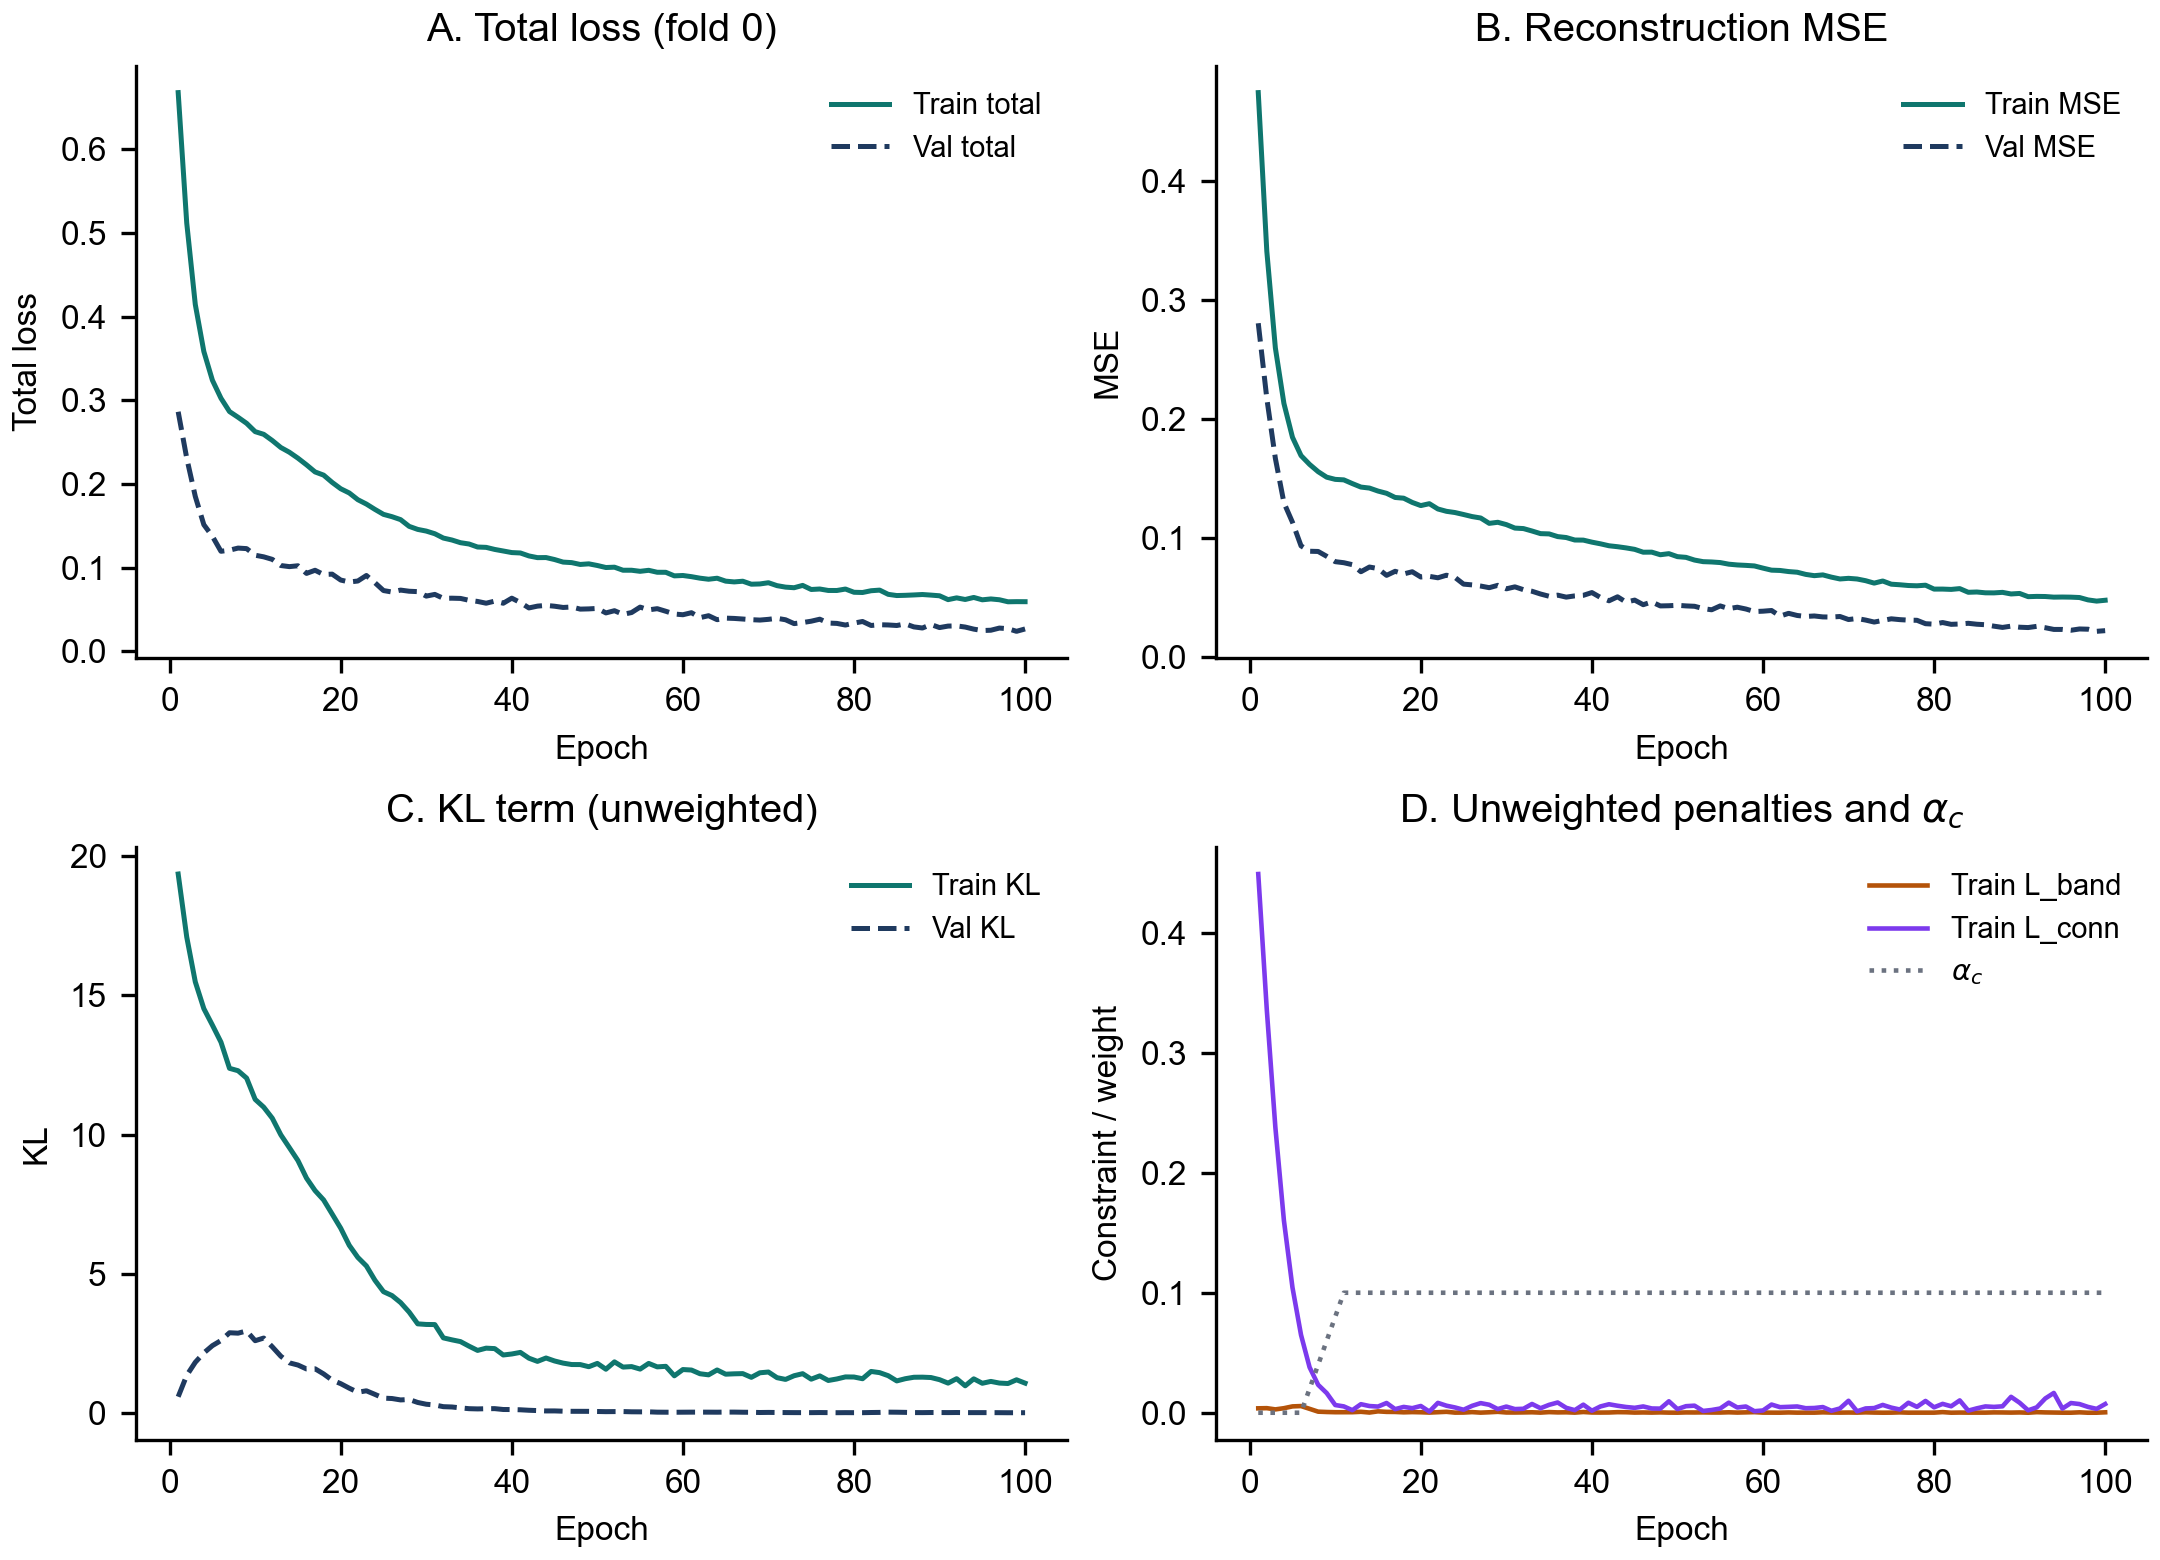
\includegraphics[width=0.95\textwidth]{figures/fig_s1_training_curves.png}
\caption{Fold-0 constrained training curves from \texttt{constrained\_evaluation\_report.json} (\texttt{constraint\_curves.fold\_0}). (A) Train and validation total loss. (B) Reconstruction MSE. (C) Unweighted KL. (D) Unweighted $L_{\mathrm{band}}$ and $L_{\mathrm{conn}}$ with the implemented $\alpha_c(t)$ schedule. Validation total loss remains below training total loss on this fold (minimum validation total $0.0241$ at epoch 99). Logged $\alpha_c$ is 0 through epoch 6 and $0.1$ by epoch 11. Alternate-seed curves were not stored. Logged values only; not an external-generalization claim.}
\label{fig:traincurves}
\end{figure*}
 Alternate-seed loss histories were not found in that report. The figure is a convergence diagnostic, not an external-performance claim.


\subsection{Regeneration entry points}

\begin{itemize}
  \item \texttt{eeg\_\allowbreak{}twin/\allowbreak{}Scripts/\allowbreak{}python.\allowbreak{}exe -m src.\allowbreak{}validation.\allowbreak{}run\_\allowbreak{}prior\_\allowbreak{}only\_\allowbreak{}direction}
  \item \texttt{eeg\_\allowbreak{}twin/\allowbreak{}Scripts/\allowbreak{}python.\allowbreak{}exe -m src.\allowbreak{}validation.\allowbreak{}compute\_\allowbreak{}direction\_\allowbreak{}r\_\allowbreak{}cis}
  \item \texttt{eeg\_\allowbreak{}twin/\allowbreak{}Scripts/\allowbreak{}python.\allowbreak{}exe -m src.\allowbreak{}validation.\allowbreak{}run\_\allowbreak{}unconstrained\_\allowbreak{}external\_\allowbreak{}battery}
  \item \texttt{eeg\_\allowbreak{}twin/\allowbreak{}Scripts/\allowbreak{}python.\allowbreak{}exe -m src.\allowbreak{}validation.\allowbreak{}run\_\allowbreak{}alpha\_\allowbreak{}c\_\allowbreak{}sweep --eval-only}
  \item \texttt{eeg\_\allowbreak{}twin/\allowbreak{}Scripts/\allowbreak{}python.\allowbreak{}exe -m src.\allowbreak{}validation.\allowbreak{}run\_\allowbreak{}delong\_\allowbreak{}oof\_\allowbreak{}probes}
  \item \texttt{eeg\_\allowbreak{}twin/\allowbreak{}Scripts/\allowbreak{}python.\allowbreak{}exe -m src.\allowbreak{}validation.\allowbreak{}run\_\allowbreak{}chemberta\_\allowbreak{}onehot\_\allowbreak{}ablation --eval-only}
  \item \texttt{eeg\_\allowbreak{}twin/\allowbreak{}Scripts/\allowbreak{}python.\allowbreak{}exe src/\allowbreak{}figures/\allowbreak{}make\_\allowbreak{}fig6\_\allowbreak{}constraint\_\allowbreak{}strength.\allowbreak{}py}
  \item \texttt{eeg\_\allowbreak{}twin/\allowbreak{}Scripts/\allowbreak{}python.\allowbreak{}exe src/\allowbreak{}figures/\allowbreak{}make\_\allowbreak{}graphical\_\allowbreak{}abstract.\allowbreak{}py}
\end{itemize}

See also \texttt{paper/\allowbreak{}CODE\_\allowbreak{}AVAILABILITY.\allowbreak{}md}.


\subsection{Known missing artifacts}

These items are not present in the locked record and are not invented here: locked-run training wall-clock; alternate-seed training curves; a public code URL and commit hash; the native EEG reference of the ds004504 files on disk; a supervised deep 2185-D classifier. Non-locked secondary Phase~C artifacts now exist separately: DeLong on stored OOF scores (\texttt{models/\allowbreak{}validation/\allowbreak{}delong\_\allowbreak{}oof\_\allowbreak{}probe\_\allowbreak{}results.\allowbreak{}json}) and a ChemBERTa-versus-padded-one-hot fold-0 ablation (\texttt{models/\allowbreak{}validation/\allowbreak{}chemberta\_\allowbreak{}onehot\_\allowbreak{}ablation/}). A non-locked fitted drug-conditioned linear imitation control is stored under \texttt{models/\allowbreak{}validation/\allowbreak{}linear\_\allowbreak{}direction\_\allowbreak{}baseline/} and is not a locked biological validation artifact. Table~\ref{tab:reviewer-defense} restates the corresponding scope boundaries.


\bibliography{references}

\end{document}
